\documentclass{lab_sheet}
\usepackage[defernumbers=true,sorting=none]{biblatex}
\DeclareBibliographyCategory{cited}
\AtEveryCitekey{\addtocategory{cited}{\thefield{entrykey}}}
\addbibresource{citation.bib}
\nocite{*} 
\renewcommand*{\thesubfigure}{\thefigure.\arabic{subfigure}}
\begin{document}
    \titlePage{Sequential Logic Design using VHDL}{December 4, 2020}
    \pagenumbering{gobble}
    \tableofcontents
    \pagebreak
    \listoffigures
    \pagebreak
    \lstlistoflistings
    \pagebreak
    \pagenumbering{arabic}
    \section{Introduction}
    \subsection{Sequential Logic Circuits}
    Unlike combinational logic circuits that change state depending upon the actual signals being applied to their inputs at that time, sequential logic circuits have some form of inherent "memory" built in. This means that sequential logic circuits are able to take into account their previous input state as well as those actually present. Thus, the output state of a sequential logic circuit is a function of the three states, viz. the “present input”, the “past input” and/or the “past output”. 
    \begin{figure}[H]
        \centering
        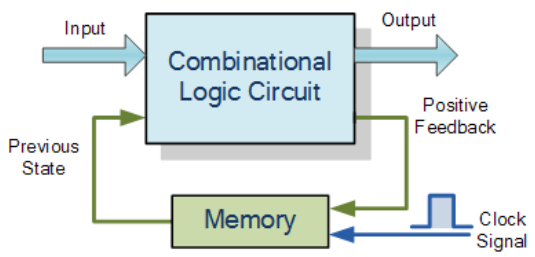
\includegraphics[]{../Figures/seq.png}
        \caption{Sequential Logic Circuit}
        \label{fig:seq}
    \end{figure}
    \subsubsection{Synchronous Sequential Circuits}
    Synchronous sequential circuits use pulsed or level inputs and a clock input to drive the circuit (with restrictions on pulse width and circuit propagation).
    \subsubsection{Asynchronous Sequential Circuits}
    Asynchronous sequential circuits do not use a clock signal as synchronous circuits do, instead the circuit is driven by the pulses of the inputs.
    \subsection{VHDL Basics}
    VHDL stands for Very High-Speed Integration Circuit HDL (Hardware Description Language). It is an IEEE (Institute of Electrical and Electronics Engineers) standard hardware description language that is used to describe and simulate the behavior of complex digital circuits. VHDL also includes design management features, and features that allow precise modeling of events that occur over time.
    \section{Objectives}
    The primary objectives of this lab experiment is to understand programming concepts in VHDL for a Field Programmable Gate Array(FPGA). VHDL coding concepts for a FPGA will enable us to write codes capable of:
    \begin{itemize}
        \item Implementing sequential circuits.
        \item Implementing test benches to verify the working of sequential circuits.
    \end{itemize}
    \section{Lab Experiment Environment}
    The lab experiments were performed virtually via simulation softwares. The basic usages of these tools will allow us to write, simulate and synthesize sequential circuts.
    \subsection{Xilinx ISE (Integrated Synthesis Environment) Design Suite}
    Xilinx ISE (Integrated Synthesis Environment) is a discontinued software tool from Xilinx for synthesis and analysis of HDL designs. It enables the developer to synthesize their designs, perform timing analysis, examine RTL diagrams, simulate a design's reaction to different stimuli, and configure the target device with the programmer. VHDL test benches are simulated on the ISE Simulator that provides a full-featured HDL simulator.
    \section{Lab Problems}
    \problem{Write a VHDL code to implement a JK flip-flop using a D flip-flop and the characteristic equation given in equation 1. The D flip-flop needs to be implemented using a structural architecture style using the circuit shown in figure below. The JK ip-op must be constructed using a component declaration for a D flip-flop. Write a VHDL test bench to verify the operation of the JK ip-op and provide waveforms.}
    The JK flip flop takes two input namely J and K that are used for setting, reseting, toggling or retaining states on the flip flop. For a D flip flop to be used as a JK flip flop, the following equation must be implemented,
    \begin{equation*}
        D=JQ'+K'Q
    \end{equation*}
    \begin{figure}[H]
        \centering
        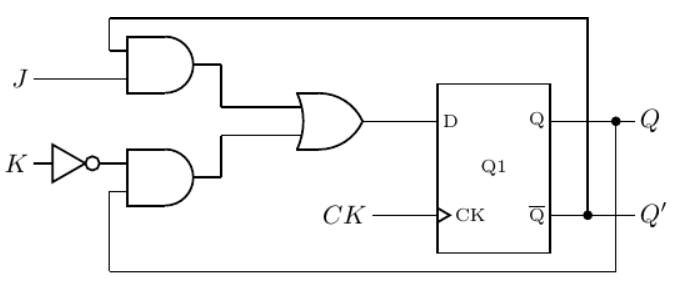
\includegraphics[]{../Figures/q1.png}
        \caption{JK flip flop using D flip flop}
        \label{fig:q1}
    \end{figure}
    \vhdlseq{jkff}{J-K flipflop implementation}{
        \vhdltwocol{combinational.vhd}{../Codes/combinational.vhd}
        \begingroup
        \captionof{lstlisting}{Combination circuit implementation: Dataflow model}
        \endgroup
        \vhdltwocol{nand\_2.vhd}{../Codes/nand_2.vhd}
        \begingroup
        \captionof{lstlisting}{2-input NAND gate implementation: Dataflow model}
        \endgroup
        \vhdltwocol{nand\_3.vhd}{../Codes/nand_3.vhd}
        \begingroup
        \captionof{lstlisting}{3-input NAND gate implementation: Dataflow model}
        \endgroup
        \vhdltwocol{dff.vhd}{../Codes/dff.vhd}
        \begingroup
        \captionof{lstlisting}{D flipflop implementation: Structural model}
        \endgroup
    }

    \problem{Write a VHDL code to implement a T flip-flop using a D flip-flop and the characteristic equation. The D flip-flop needs to be implemented using a structural architecture style using the circuit shown in below figure. The T flip-flop must be constructed using a component declaration for a D flip-flop. Write a VHDL test bench to verify the operation of the T flip-flop and provide waveforms.}
    \begin{figure}[H]
        \centering
        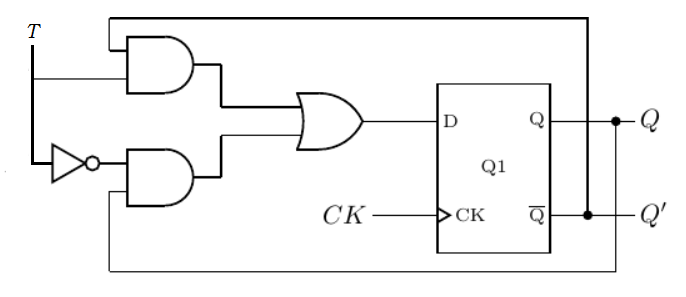
\includegraphics[scale=1]{../Figures/q2.png}
        \caption{T flip flop using D flip flop}
        \label{fig:q2}
    \end{figure}
    T flip flop, or also known as the toggle flip flop complements the output if the input T is high, else retains the state. For a D flip flop to be used as a T flip flop, the following equation must be implemented,
    \begin{equation*}
        D=TQ'+T'Q
    \end{equation*}
    \vhdlseq{tff}{T flipflop implementation}{
    }

    \problem{Use VHDL to implement a 4-bit serial-in-serial-out (SISO) right-shift register as shown in figure below. Determine the output of the shift register after the input sequence 01010101 has been shifted eight times, starting with the MSB. Assume that the output of the shift register is reset initially to 0000. The shift register must be constructed with D flip-flops using a component declaration for a D flip-flop. Write a VHDL test bench to verify the operation of the 4-bit SISO and provide appropriate waveforms.}
    \begin{figure}[H]
        \centering
        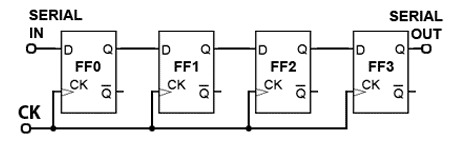
\includegraphics[]{../Figures/q3.png}
        \caption{4-bit serial-in-serial-out (SISO) right-shift register}
        \label{fig:q3}
    \end{figure}

    \vhdlseq{siso}{4-bit serial-in-serial-out right-shift register implementation}{
    }

    \problem{Write a VHDL code to implement a 4-bit synchronous up-counter as shown in below figure. In a synchronous counter all flip-flops receive a common clock signal and change their states at the same time. The shift-register must be constructed with T flip-flops using a component declaration for a T flip-flop. Write a VHDL test bench to verify the operation of the 4-bit synchronous up-counter and provide the appropriate waveforms.}
    \begin{figure}[H]
        \centering
        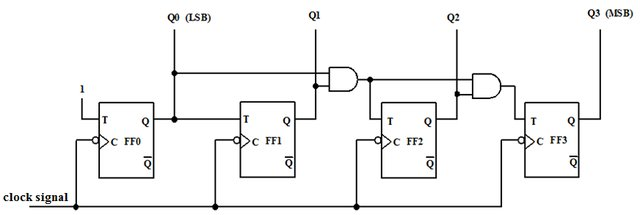
\includegraphics[width=\linewidth]{../Figures/q4.jpg}
        \caption{4-bit synchronous up counter using T flip flop}
        \label{fig:q4}
    \end{figure}

    \vhdlseq{syncup}{4-bit synchronous up counter implementation}{
        \vhdltwocol{tff\_be.vhd}{../Codes/tff_be.vhd}
        \begingroup
        \captionof{lstlisting}{T flipflop implementation: Behavioral model}
        \endgroup
    }

    \problem{Use VHDL to design an asynchronous decade counter as shown in below figure. The 10 states of a decade counter represent the BCD numbers from 0 to 9. Write the VHDL test bench to verify the operation of the decade counter and provide waveforms.}
    \begin{figure}[H]
        \centering
        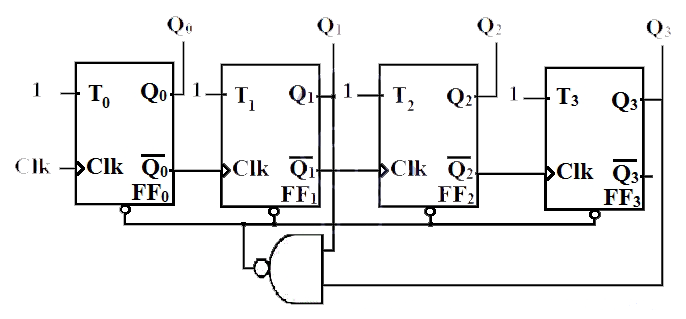
\includegraphics[width=\linewidth]{../Figures/q5.png}
        \caption{Asynchronous decade counter using T flip flop}
        \label{fig:q5}
    \end{figure}
    
    \vhdlseq{asyncdec}{4-bit asynchronous decade counter implementation}{}

    \problem{Use VHDL to design a four-bit Johnson counter as shown in below figure. The Johnson counter must be constructed using component declarations from the D flip-flops. Write a VHDL test bench to verify the operation of the Johnson counter and provide waveforms.}
    \begin{figure}[H]
        \centering
        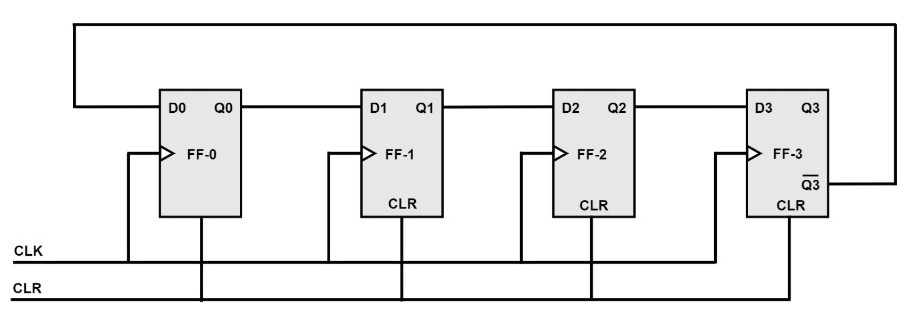
\includegraphics[scale=0.5]{../Figures/q6.jpg}
        \caption{4-bit johnson counter using D flip flop}
        \label{fig:q6}
    \end{figure}
    \vhdlseq{john}{4-bit johnson counter implementation}{
        \vhdltwocol{dff\_st.vhd}{../Codes/dff_st.vhd}
        \begingroup
        \captionof{lstlisting}{D flipflop implementation: Structural model}
        \endgroup
    }

    \problem{Use VHDL to create a 2-bit BCD counter as shown in below figure. The BCD counter consists of two 1-bit BCD counters cascaded to form a 2-bit BCD counter. The 2-bit BCD counter counts from 00 to 99. The 2-bit BCD counter must be constructed using component declarations for the D flip-flops.}
    \begin{figure}[H]
        \centering
        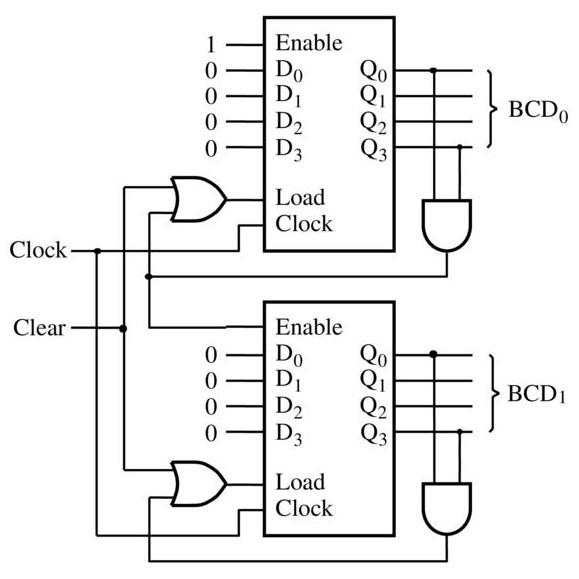
\includegraphics[scale=2.5]{../Figures/q7.jpg}
        \caption{2-bit BCD counter by cascading two 1-bit BCD counters}
        \label{fig:q7}
    \end{figure}
    \vhdlseq{q7bcd}{2-bit BCD counter implementation}{
        \vhdltwocol{q7diff.vhd}{../Codes/q7dff.vhd}
        \begingroup
        \captionof{lstlisting}{D flipflop implementation with enable pin: Structural model}
        \endgroup
    }
    \section{Observations}
    The observations for the ISim simulator are printed to individual .pdf fles using the print option available within the simulator. The time frames have been selected such that all the possible input cases are included at least once within the waveform. The expected outputs and the simulated waveform match leading us to a conclusion that the designed sequential circuits are functional. The RTL schematic for each question have been included with this report since it was also a major part of the observation. The RTL schematic shows the internal logic gates that are used starting from the top module.
    \subsubsection*{Problem 1}
    \begin{figure}[H]
        \centering
        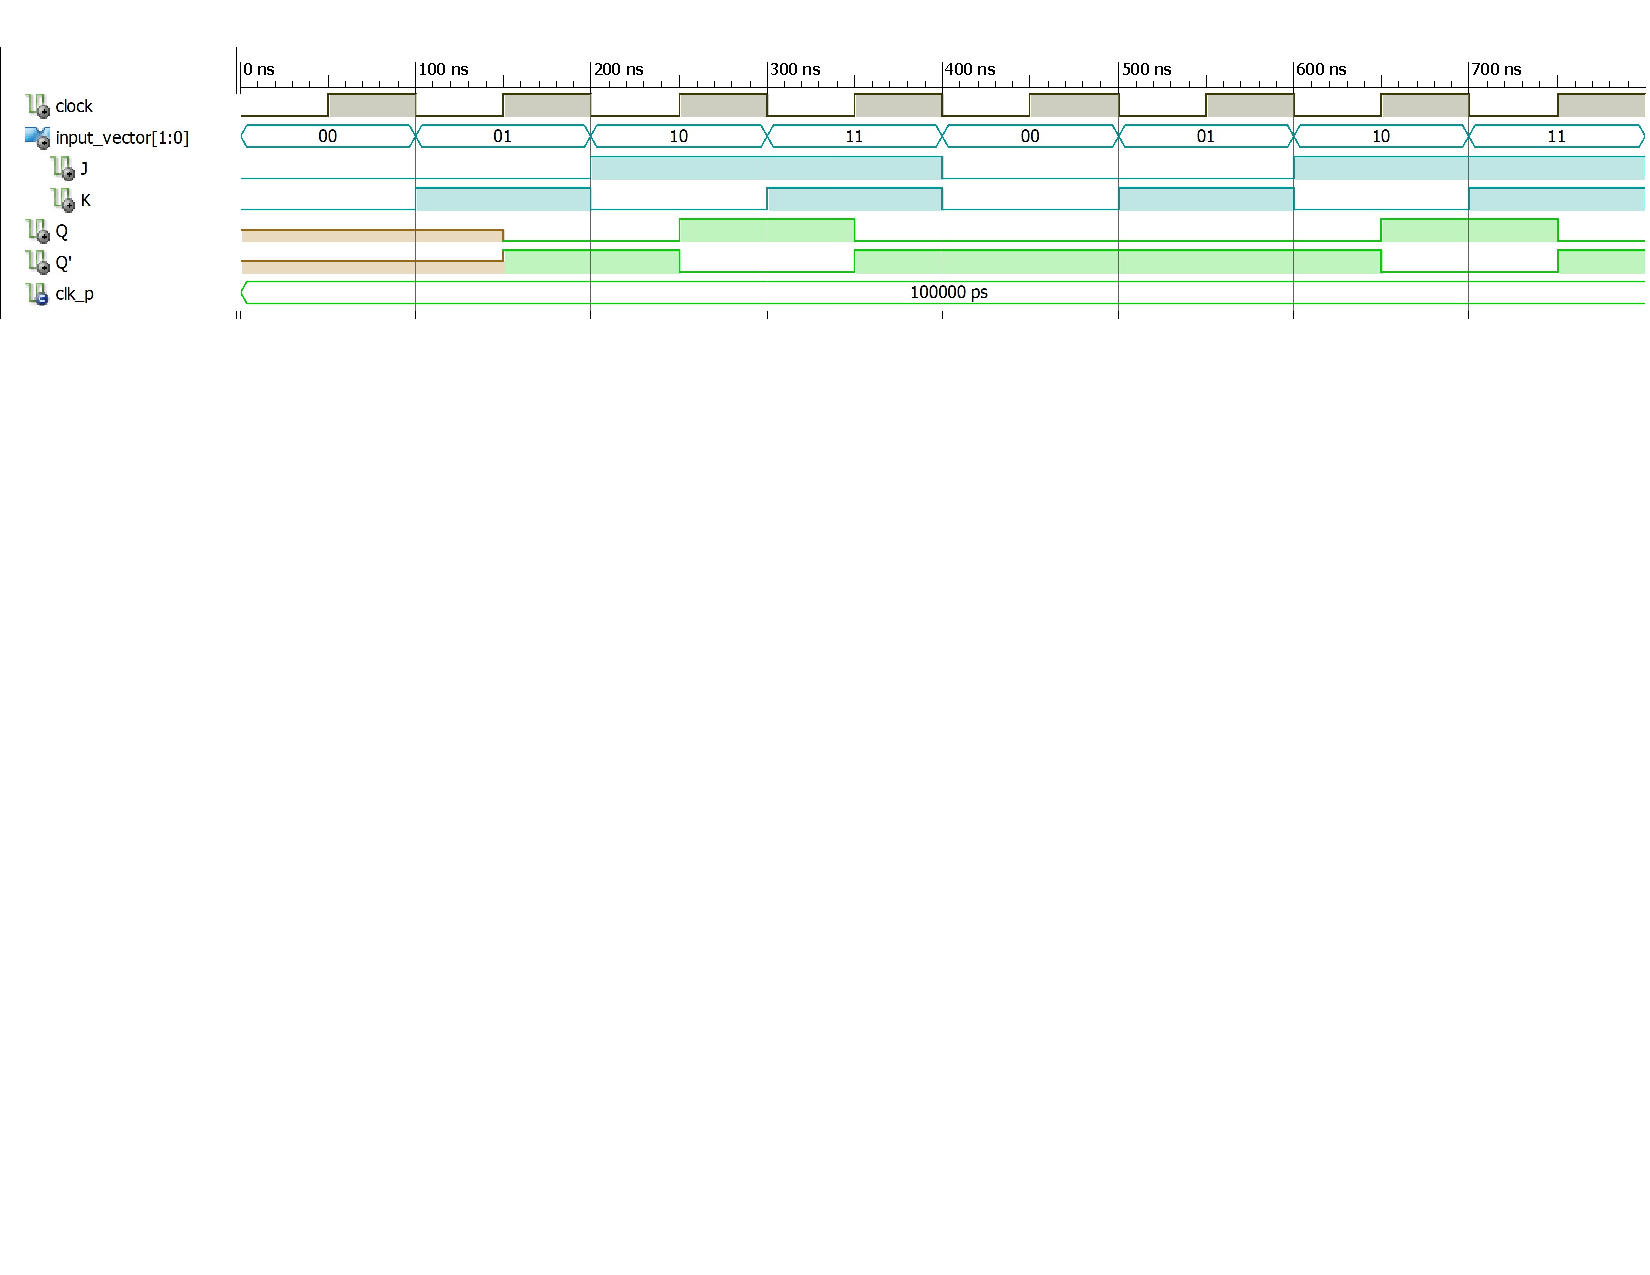
\includegraphics[width=.95\linewidth, height=30mm, frame]{../Figures/1.pdf}
        \caption{Observed waveform for Problem 1}
        \label{fig:obs1}
    \end{figure}
    \begin{figure}[H]
        \centering
        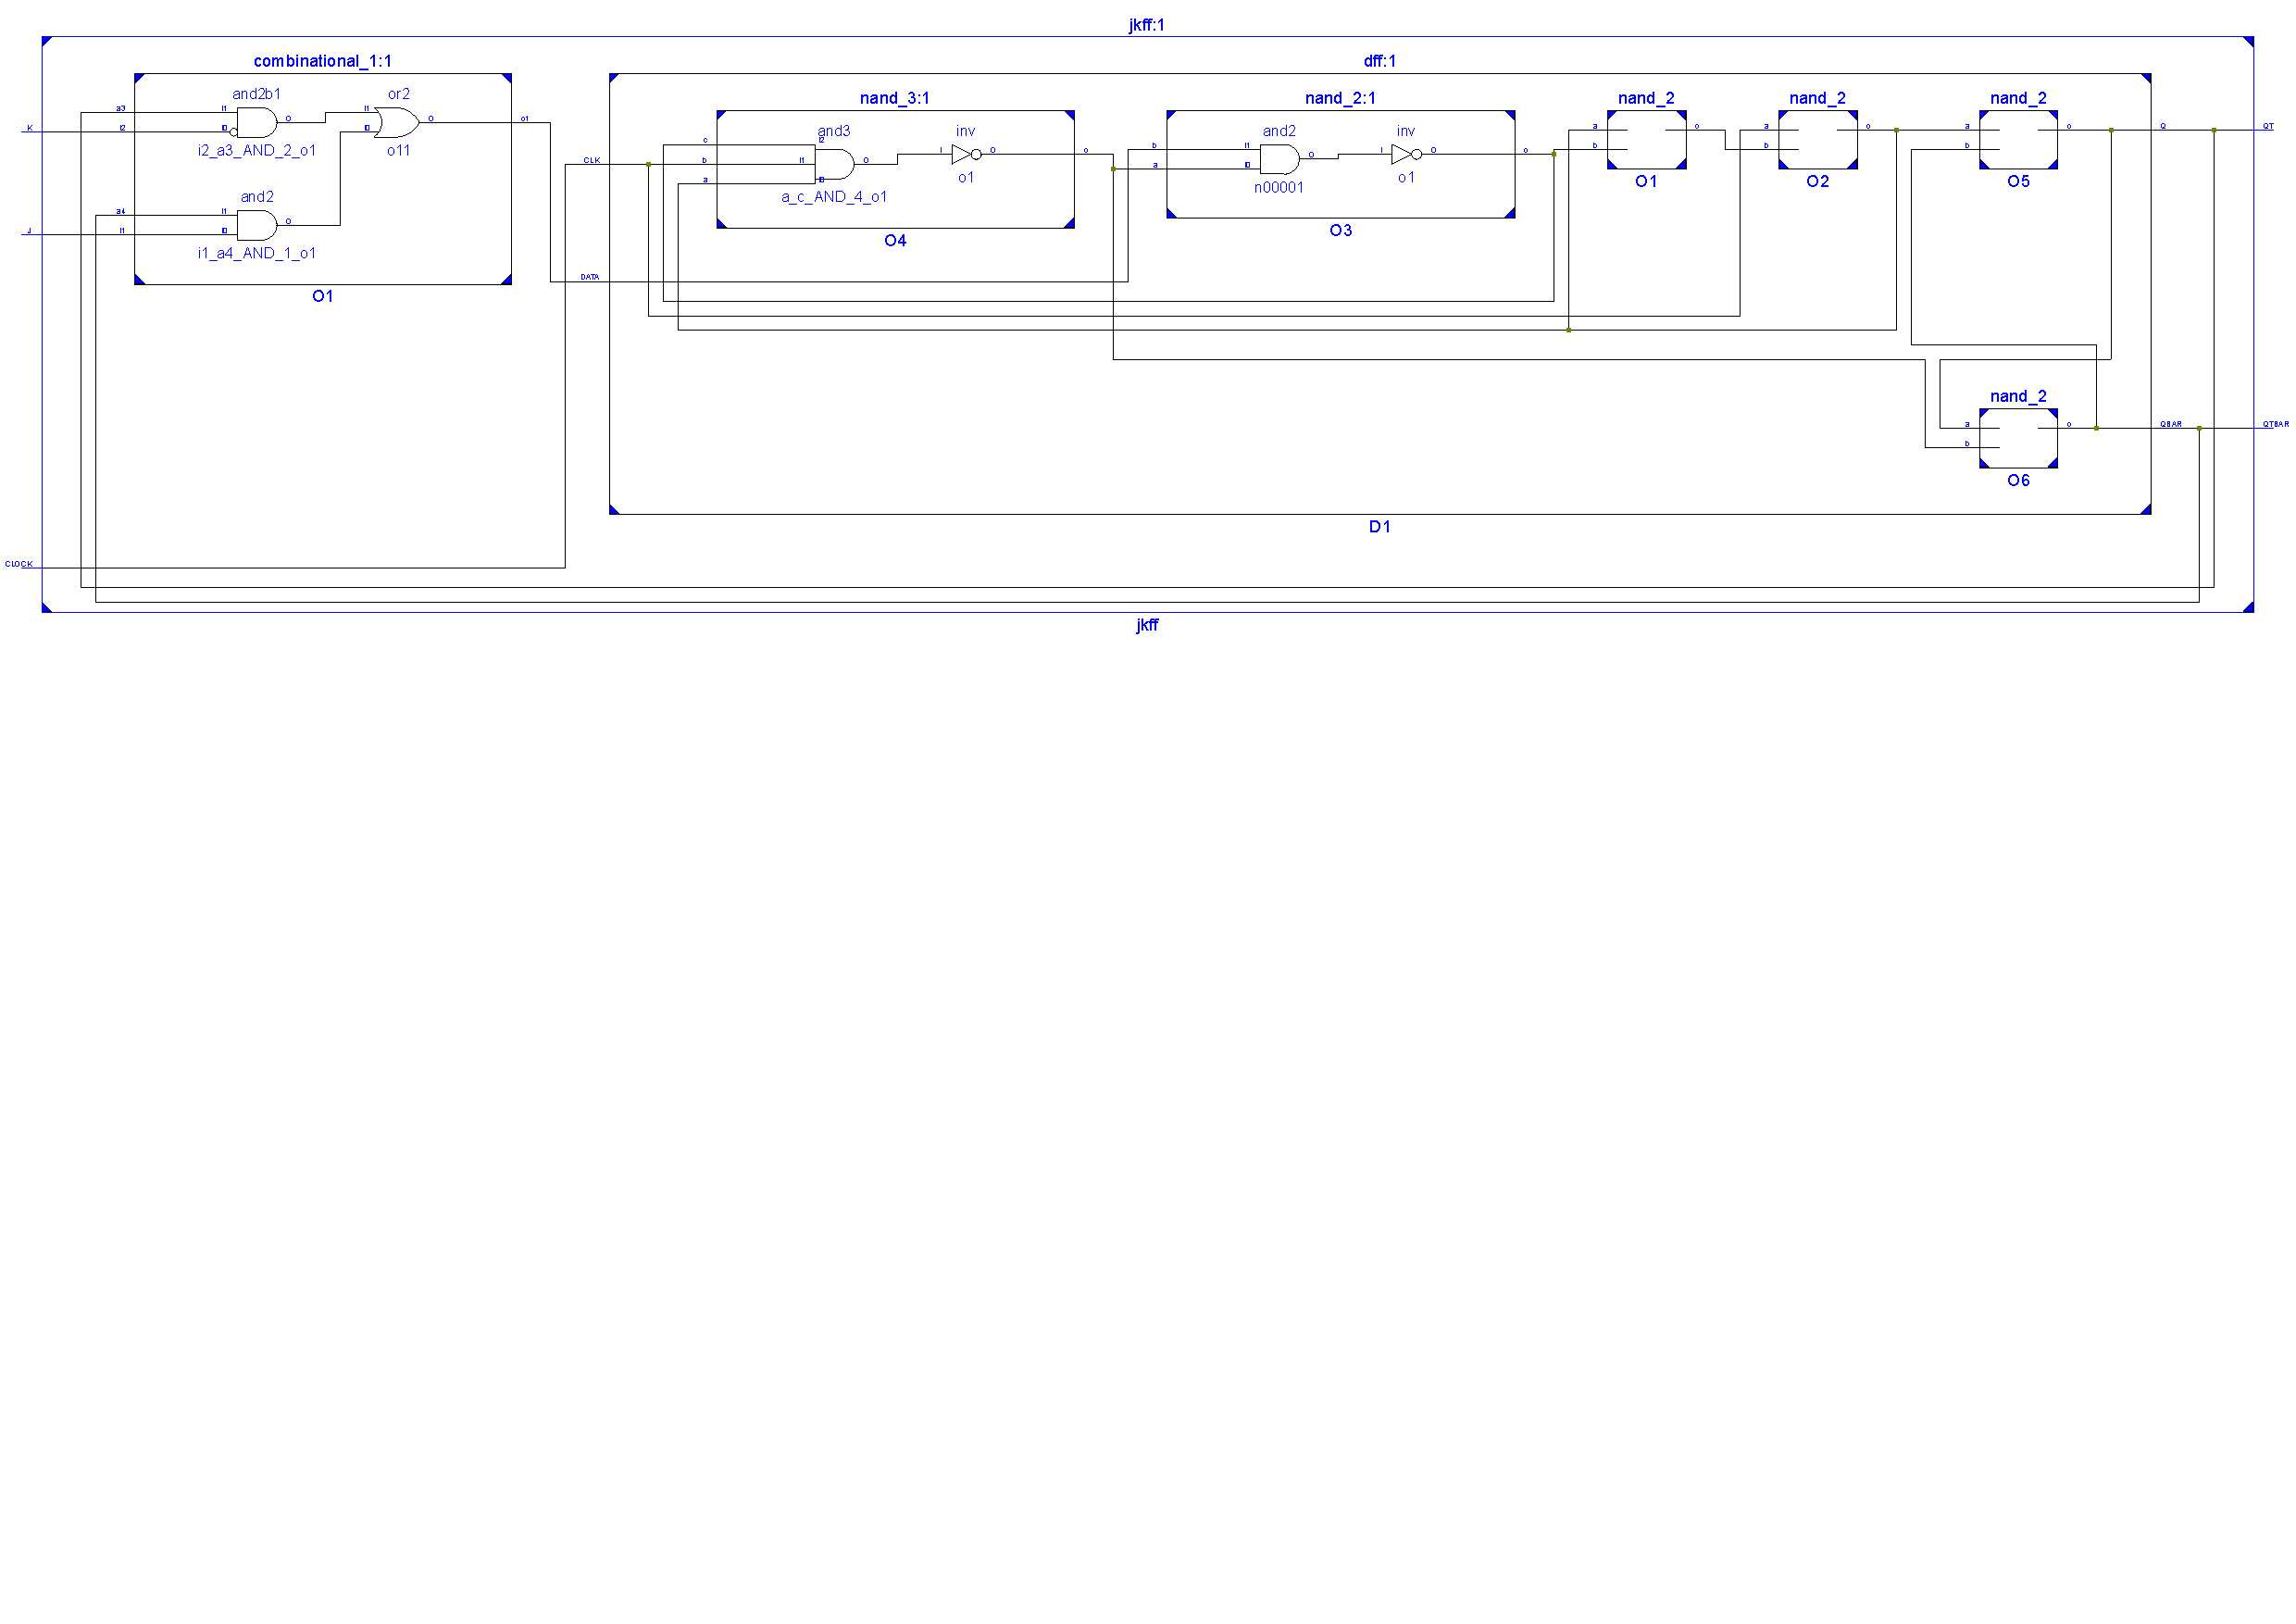
\includegraphics[width=\linewidth,  height=60mm]{../Figures/q1_ckt.pdf}
        \caption{Observed RTL schematic for Problem 1}
        \label{fig:rtl1}
    \end{figure}

    \subsubsection*{Problem 2}
    \begin{figure}[H]
        \centering
        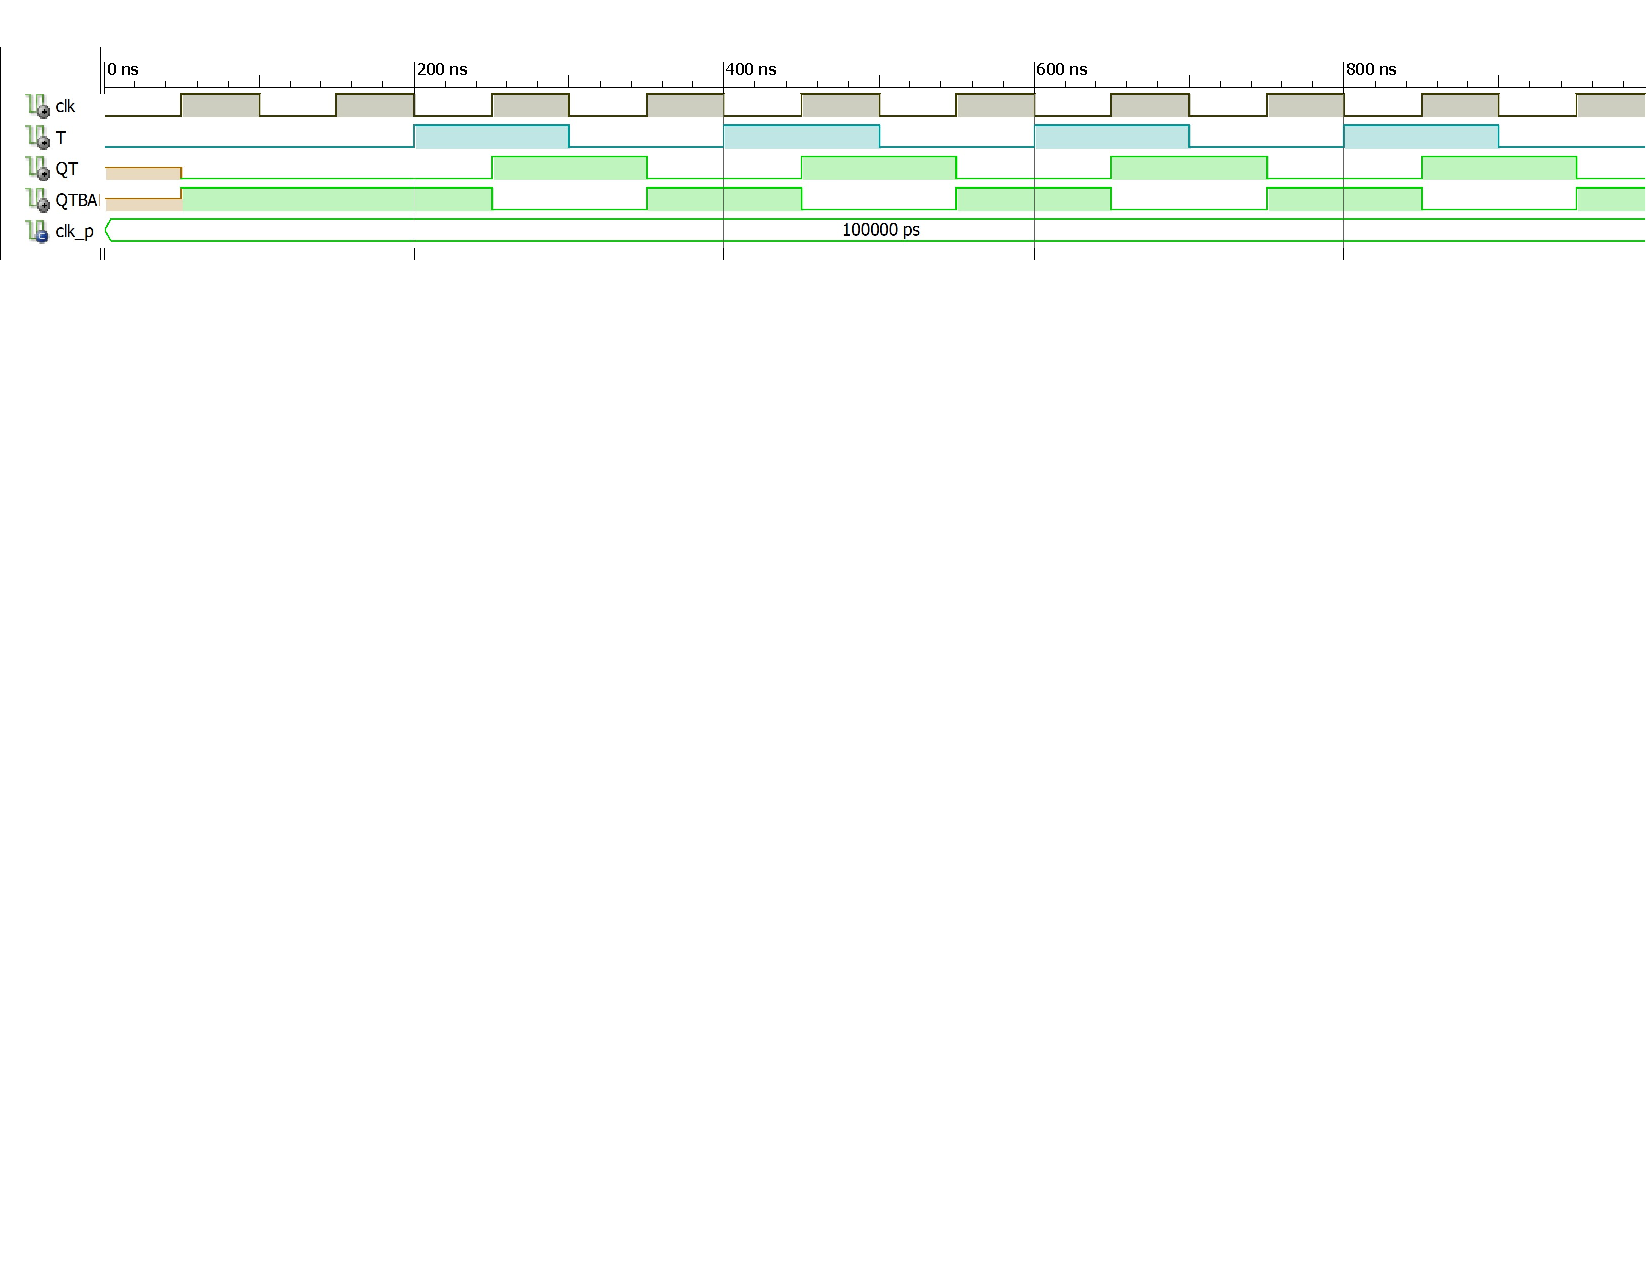
\includegraphics[width=.95\linewidth, height=30mm, frame]{../Figures/2.pdf}
        \caption{Observed waveform for Problem 2}
        \label{fig:obs2}
    \end{figure}
    \begin{figure}[H]
        \centering
        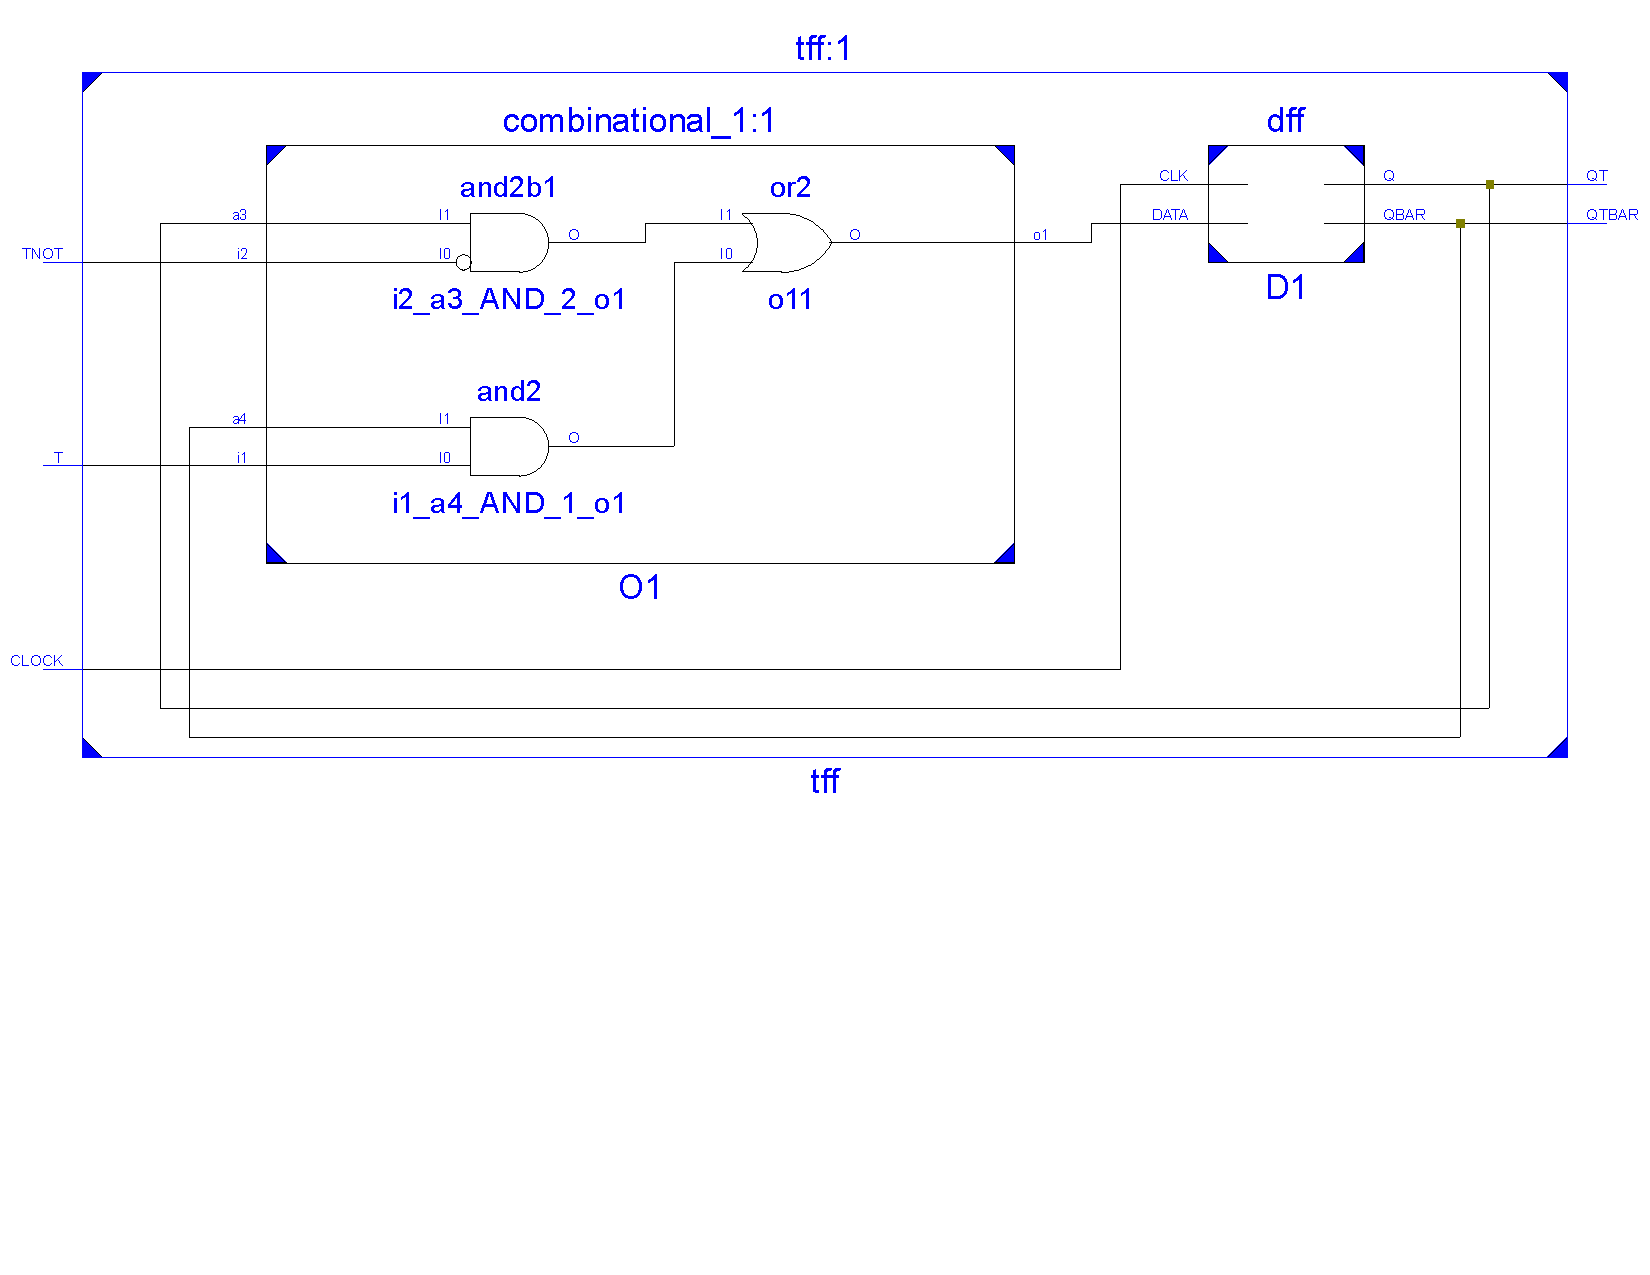
\includegraphics[scale=0.5]{../Figures/q2_ckt.pdf}
        \caption{Observed RTL schematic for Problem 2}
        \label{fig:rtl2}
    \end{figure}

    \subsubsection*{Problem 3}
    \begin{figure}[H]
        \centering
        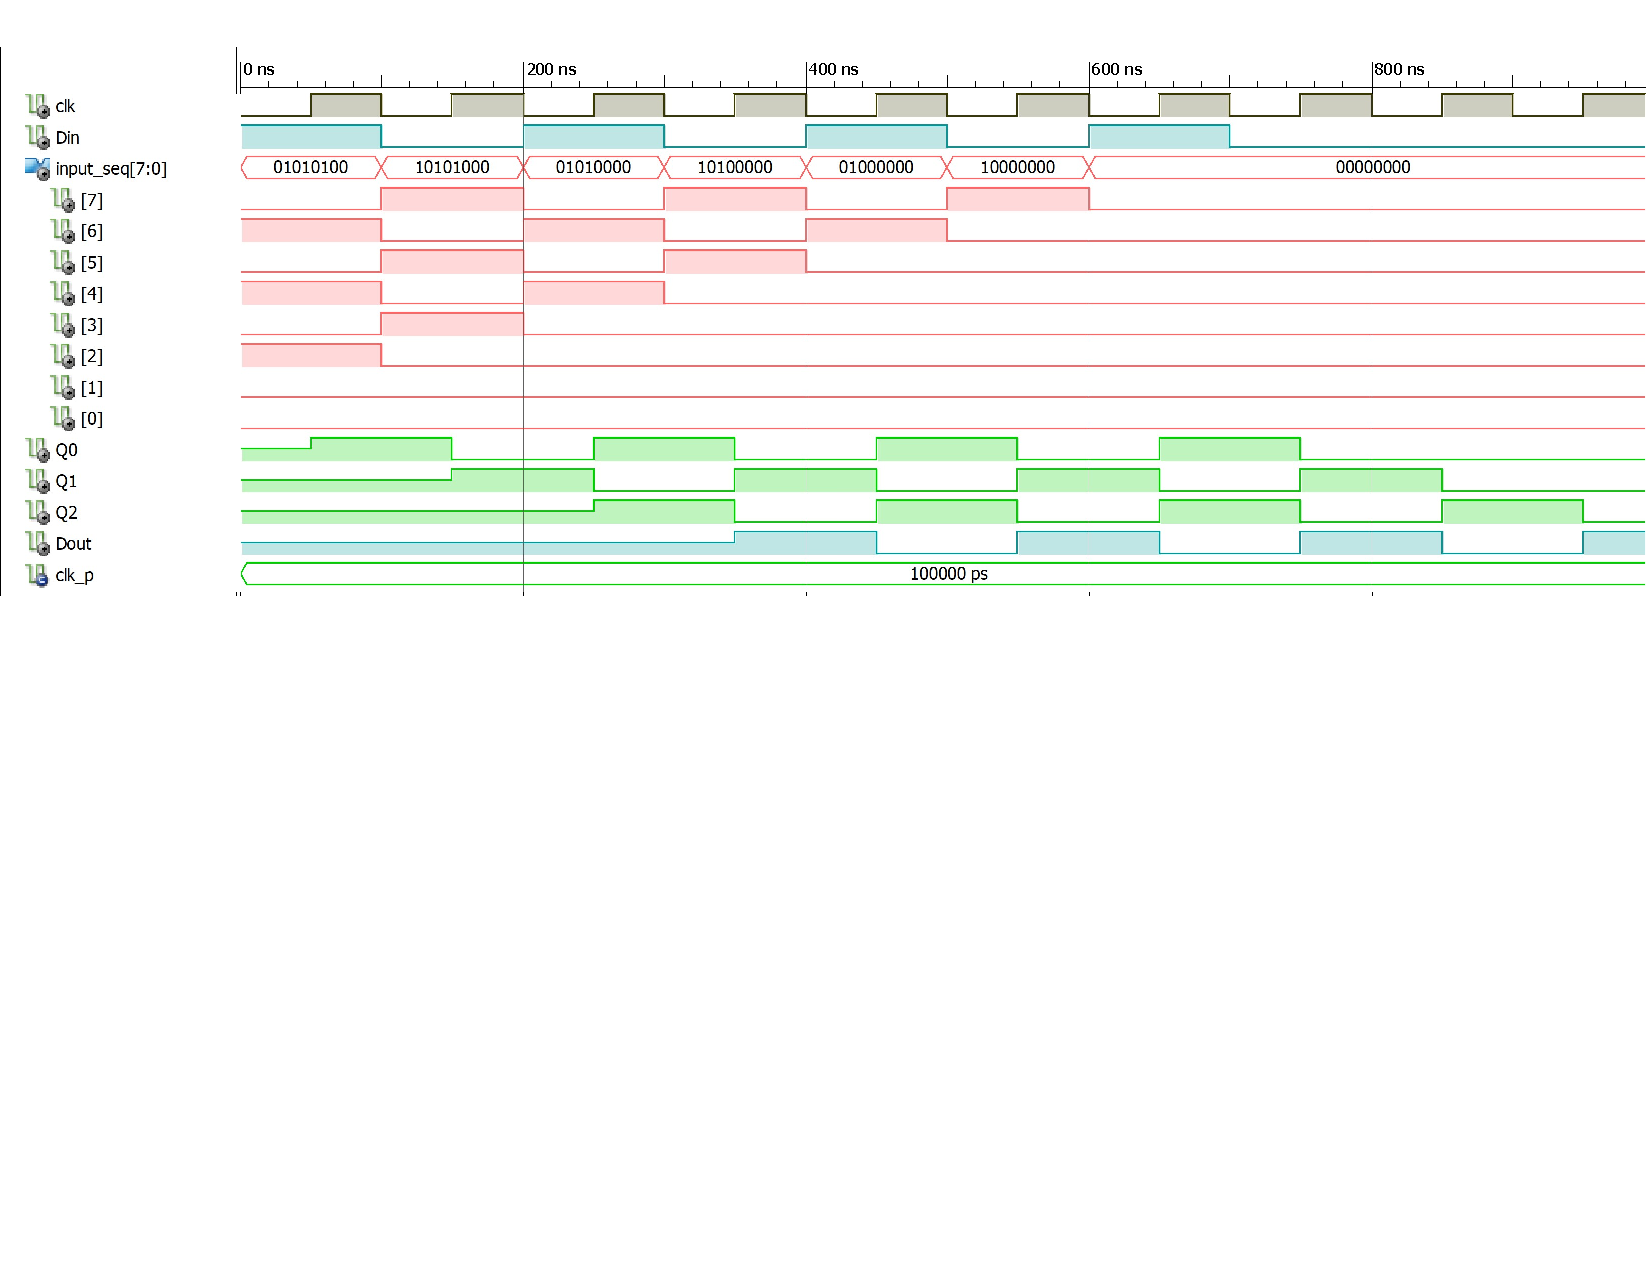
\includegraphics[width=.95\linewidth, frame]{../Figures/3.pdf}
        \caption{Observed waveform for Problem 3}
        \label{fig:obs3}
    \end{figure}
    \begin{figure}[H]
        \centering
        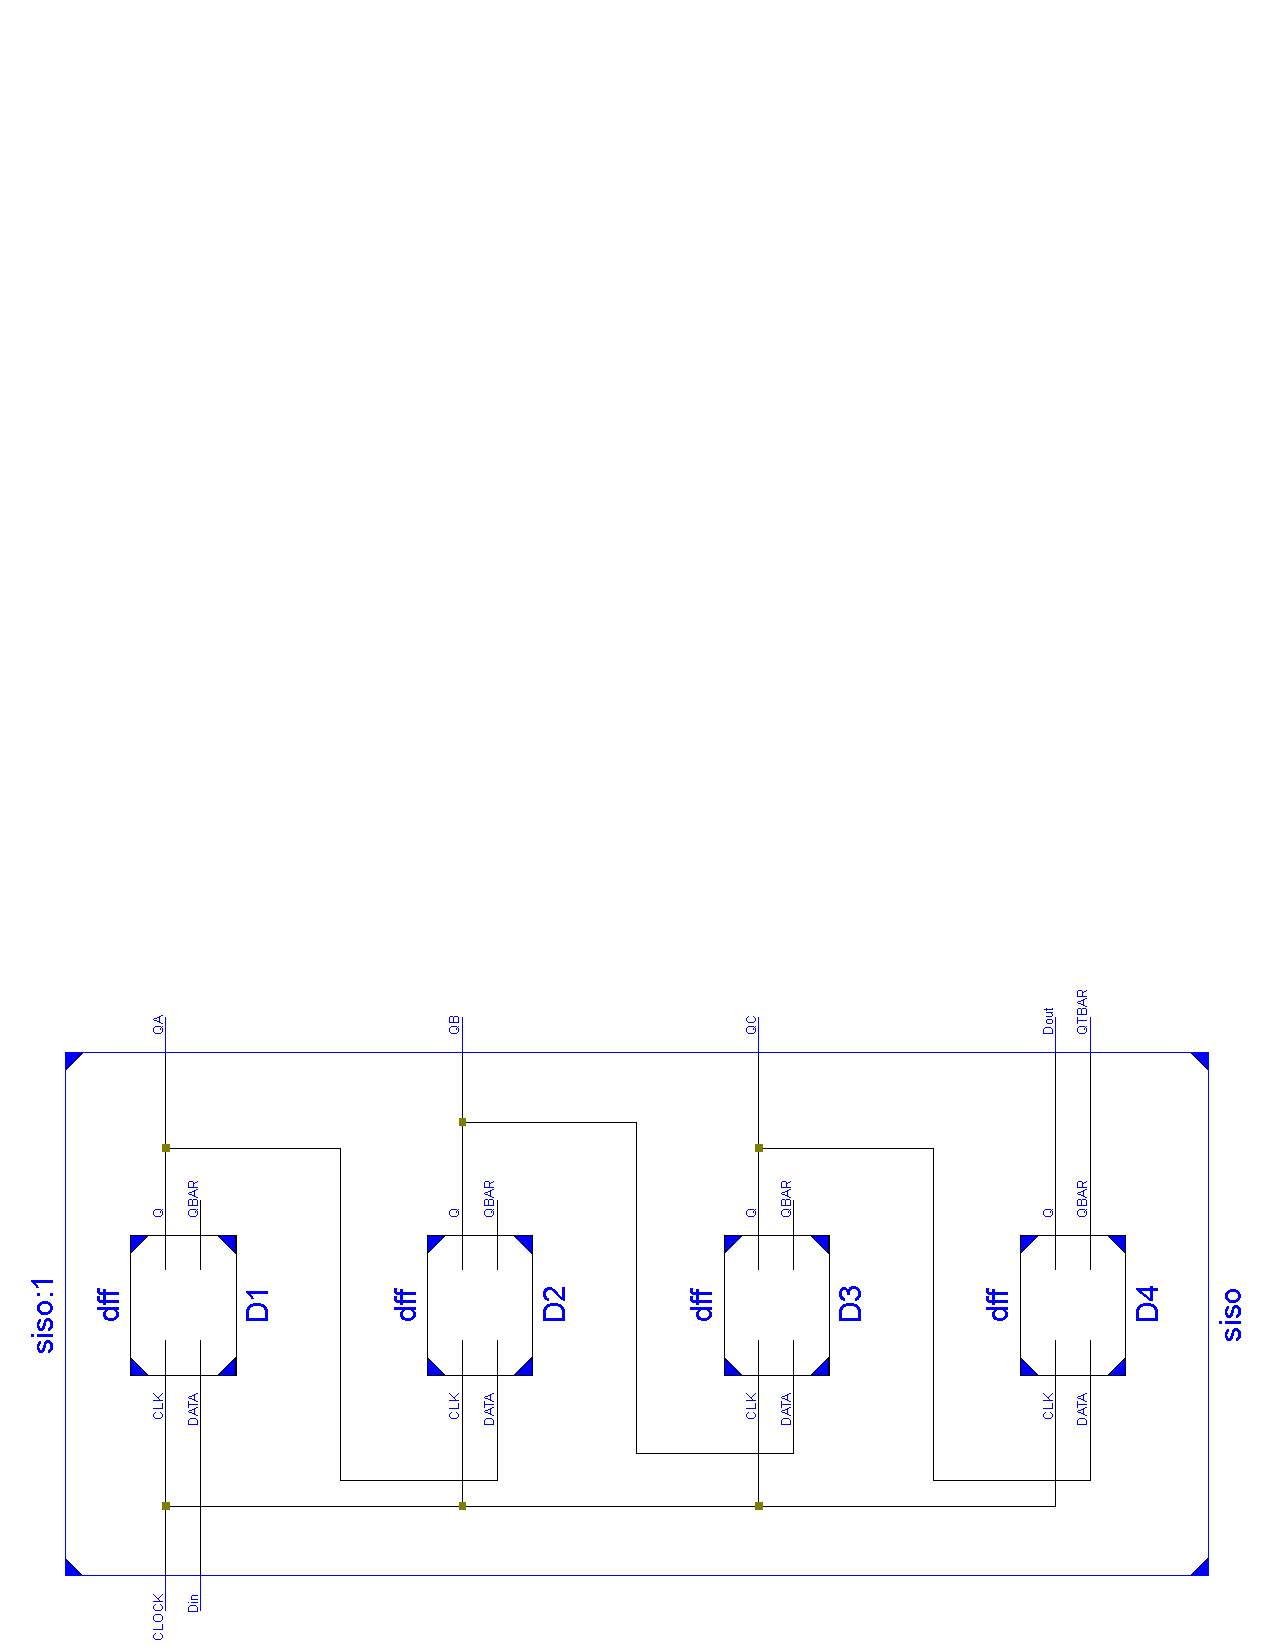
\includegraphics[scale=0.5]{../Figures/q3_ckt.pdf}
        \caption{Observed RTL schematic for Problem 3}
        \label{fig:rtl3}
    \end{figure}

    \subsubsection*{Problem 4}
    \begin{figure}[H]
        \centering
        \begin{subfigure}{\linewidth}
            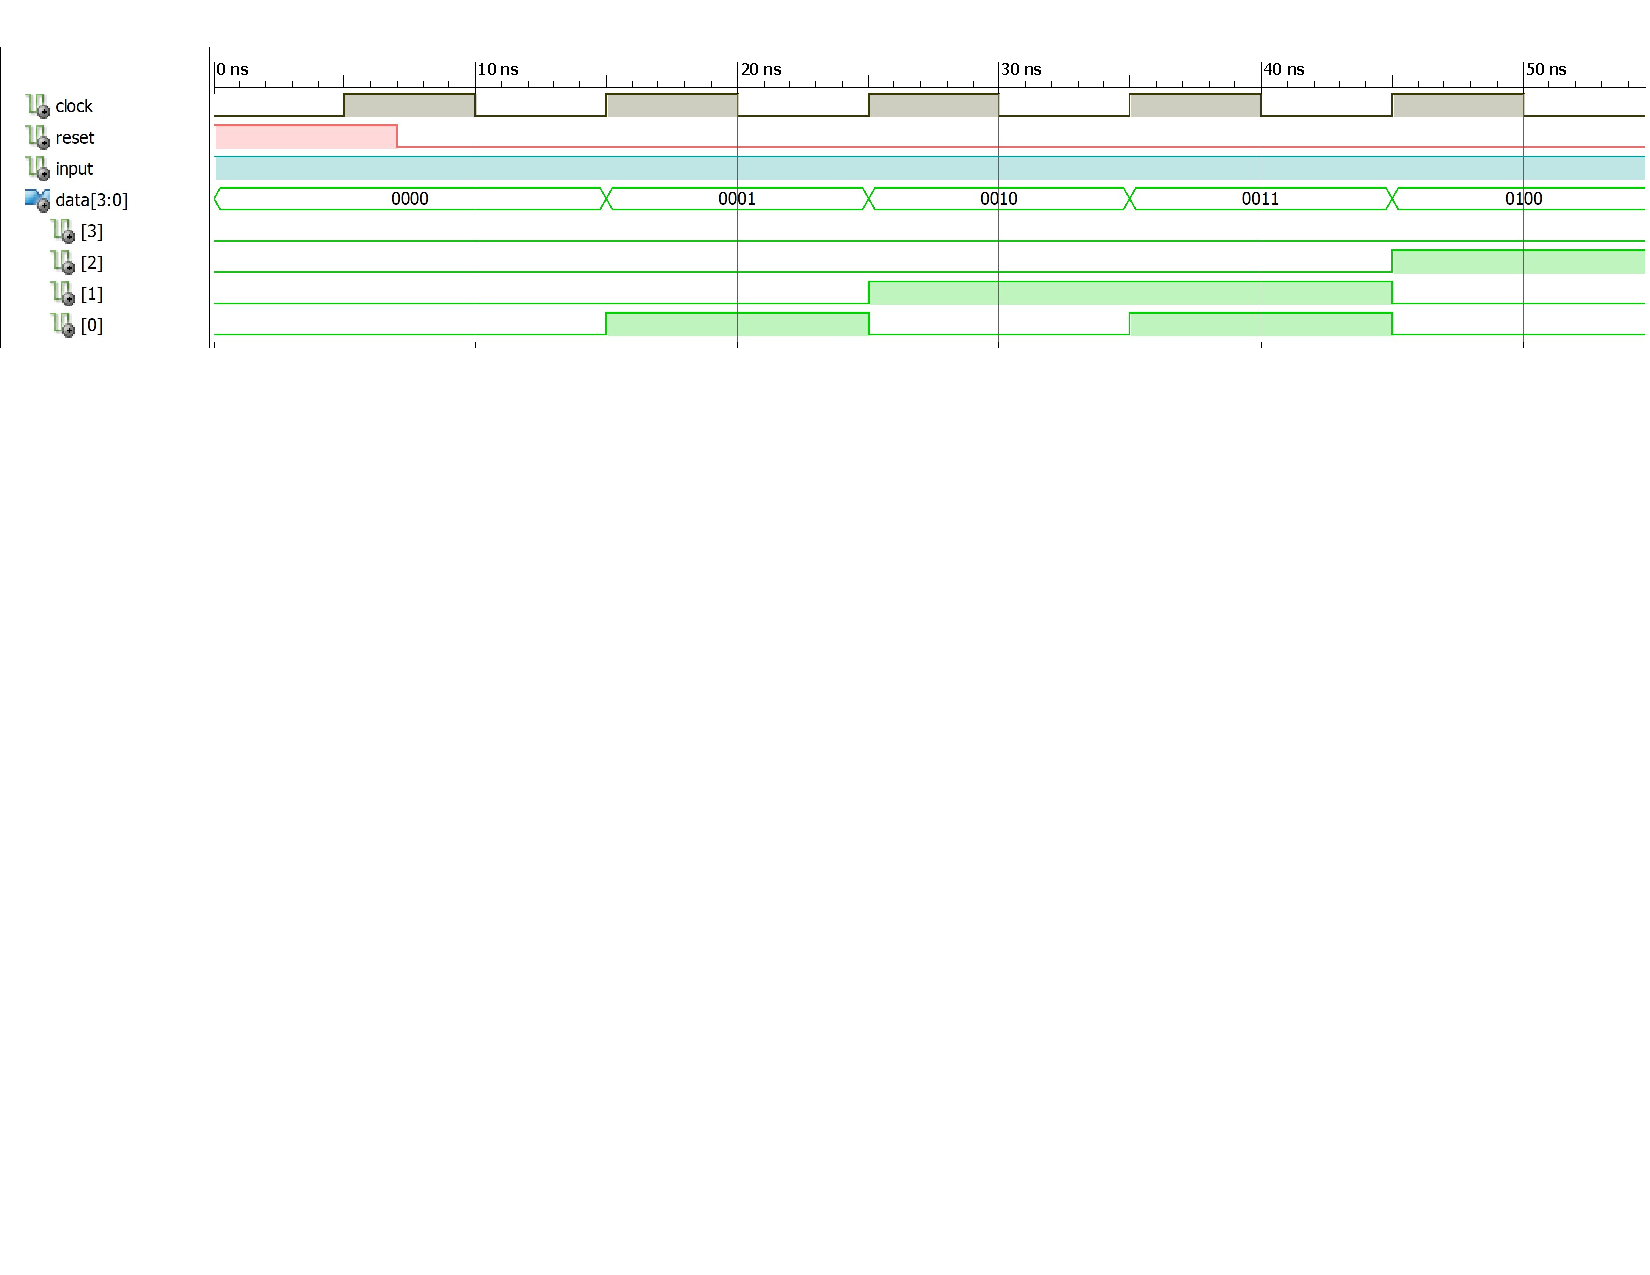
\includegraphics[width=.95\linewidth, frame]{../Figures/4-1.pdf}
        \caption{}
        \label{fig:obs4-1}
        \end{subfigure}
        \begin{subfigure}{\linewidth}
            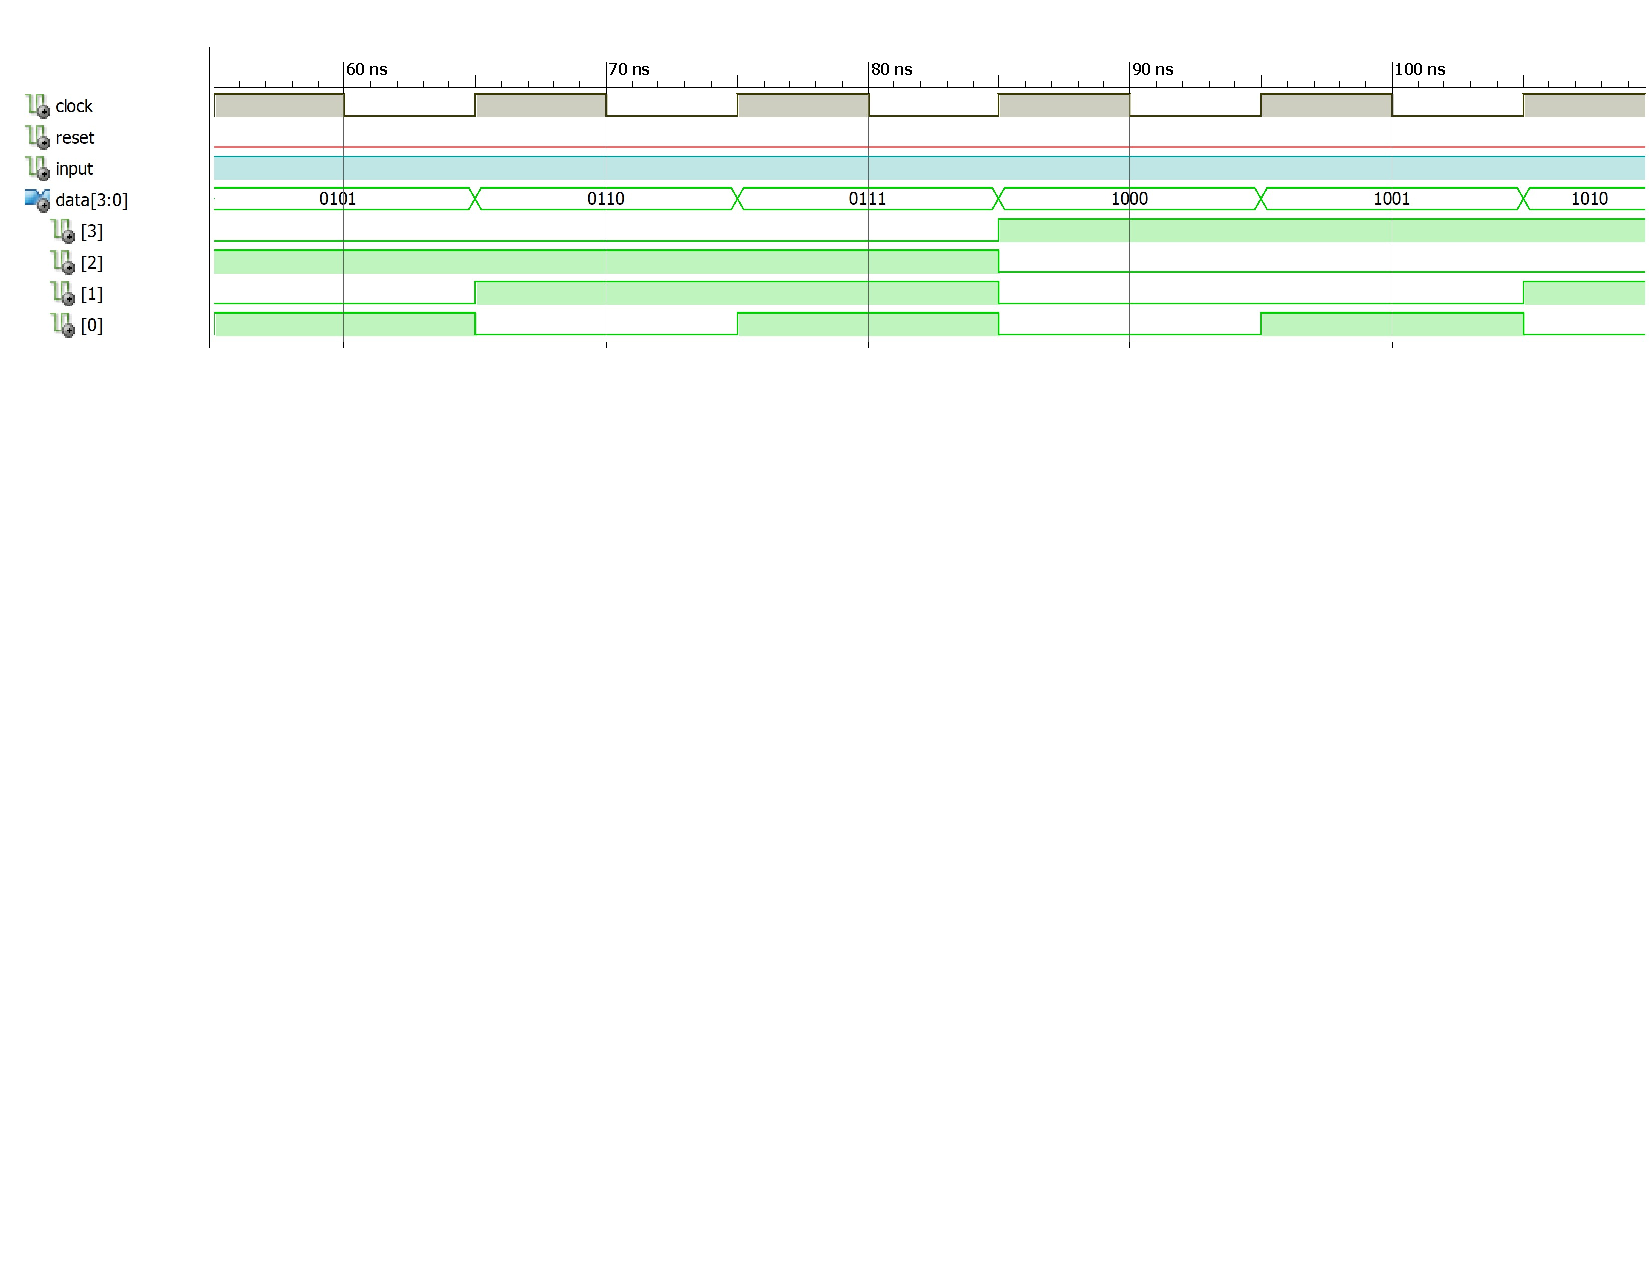
\includegraphics[width=.95\linewidth, frame]{../Figures/4-2.pdf}
        \caption{}
        \label{fig:obs4-2}
        \end{subfigure}
        \begin{subfigure}{\linewidth}
            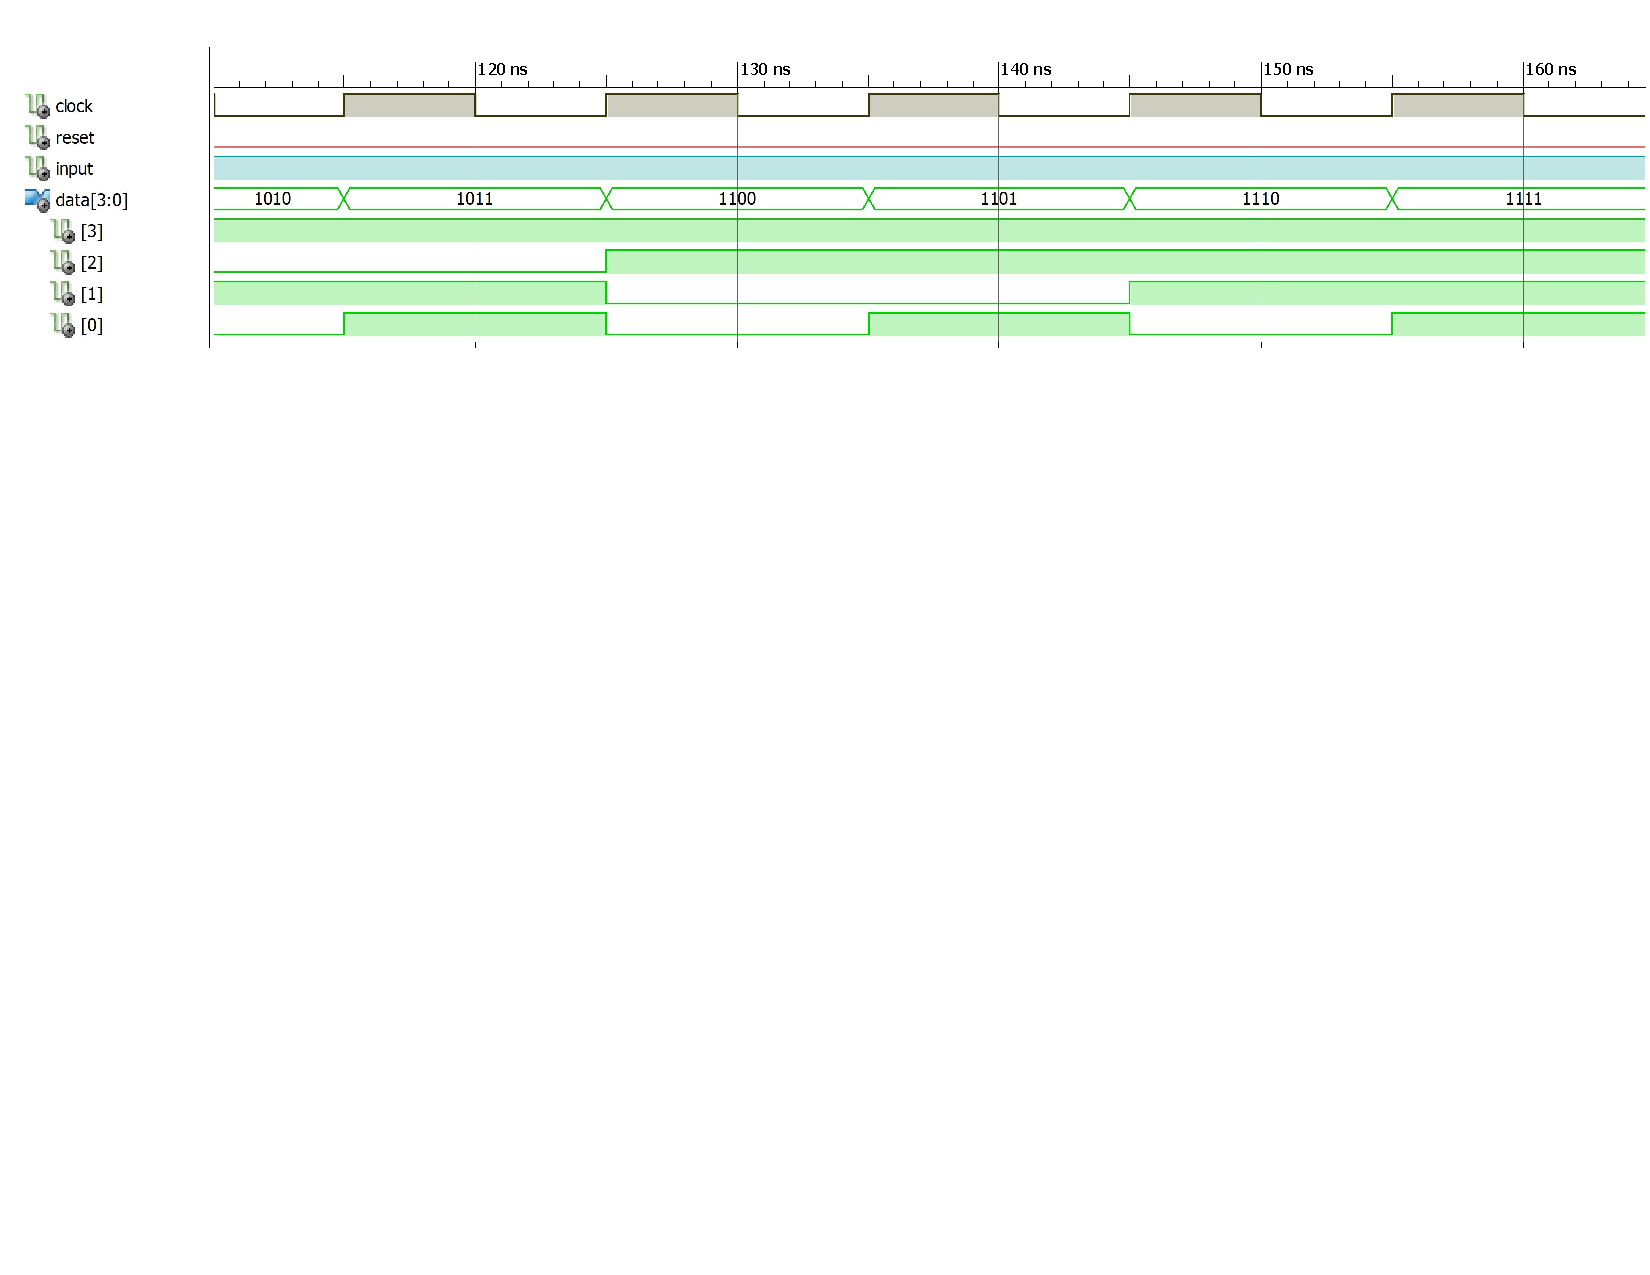
\includegraphics[width=.95\linewidth, frame]{../Figures/4-3.pdf}
        \caption{}
        \label{fig:obs4-3}
        \end{subfigure}
        \caption{Observed waveform for Problem 4}
        \label{fig:obs4}
    \end{figure}
    \begin{figure}[H]
        \centering
        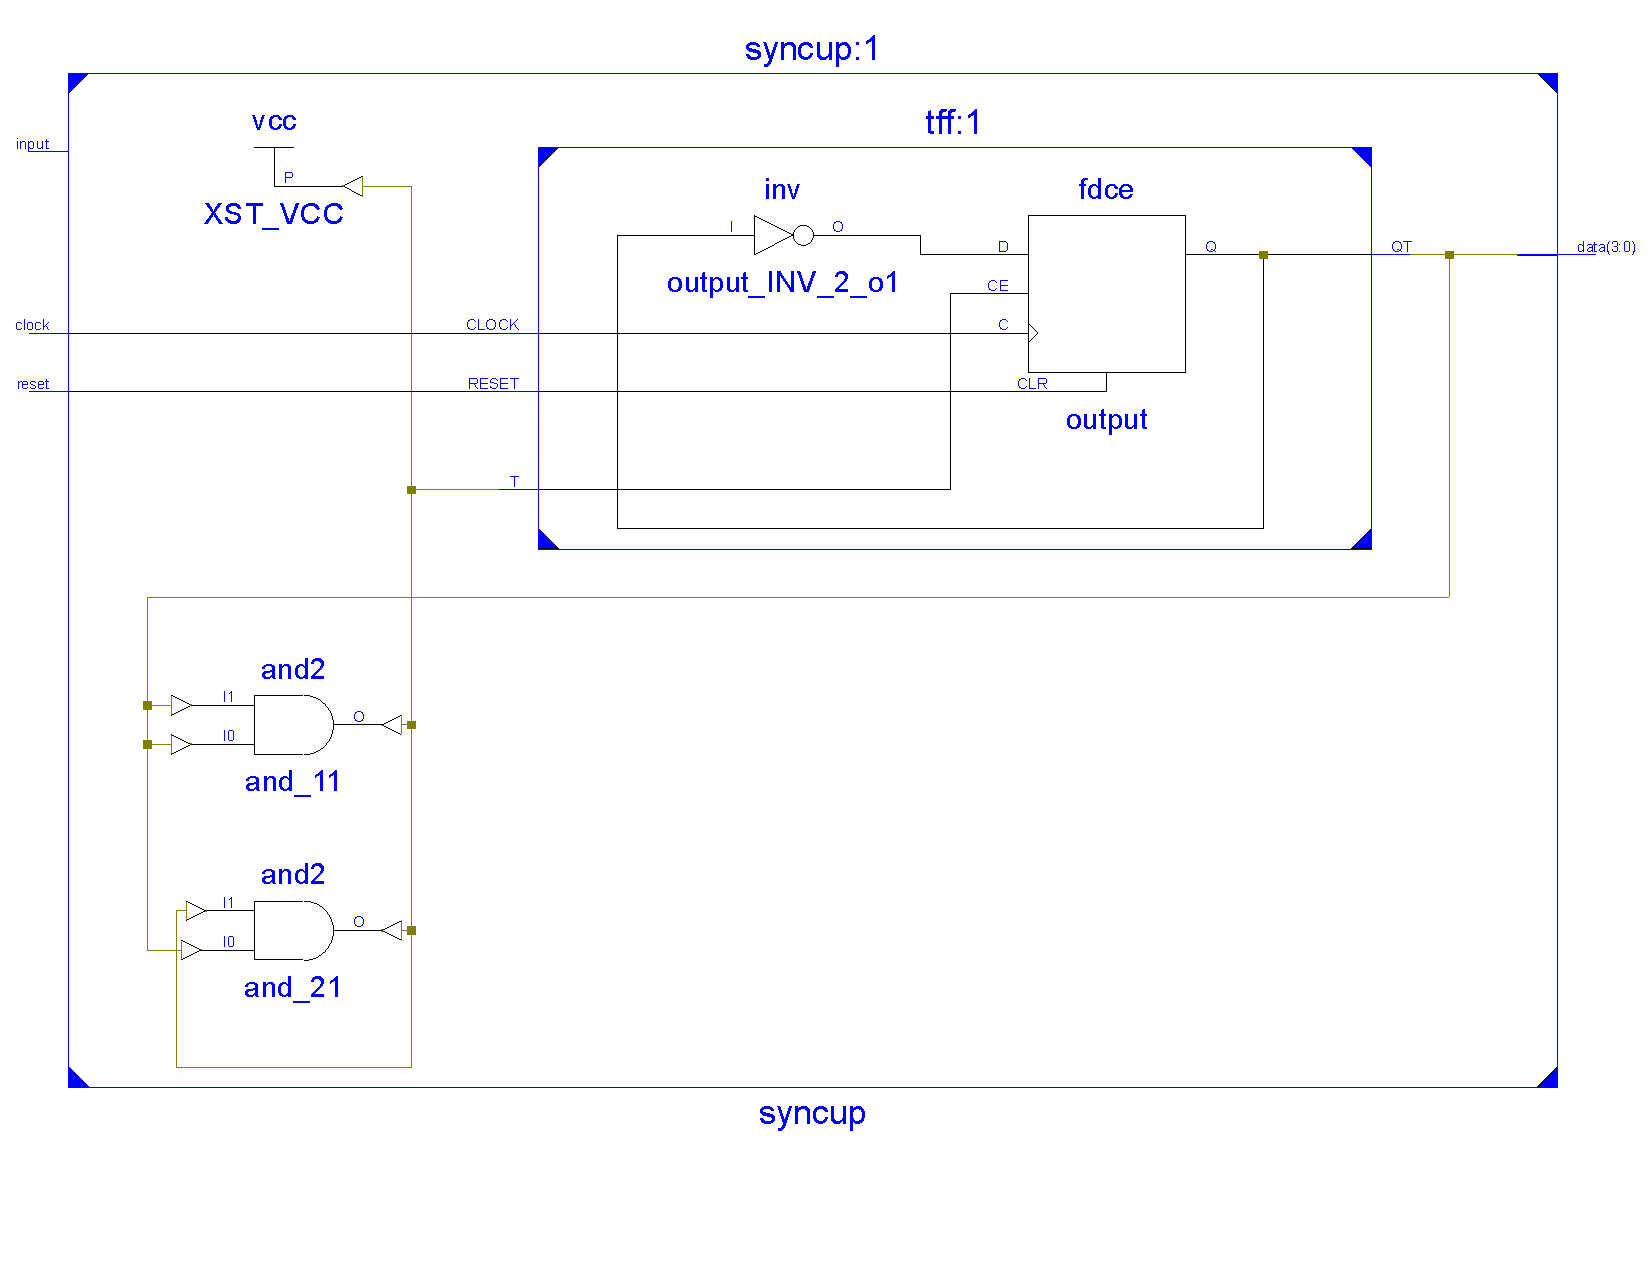
\includegraphics[scale=0.4]{../Figures/q4_ckt.pdf}
        \caption{Observed RTL schematic for Problem 4}
        \label{fig:rtl4}
    \end{figure}

    \subsubsection*{Problem 5}
    \begin{figure}[H]
        \centering
        \begin{subfigure}{\linewidth}
            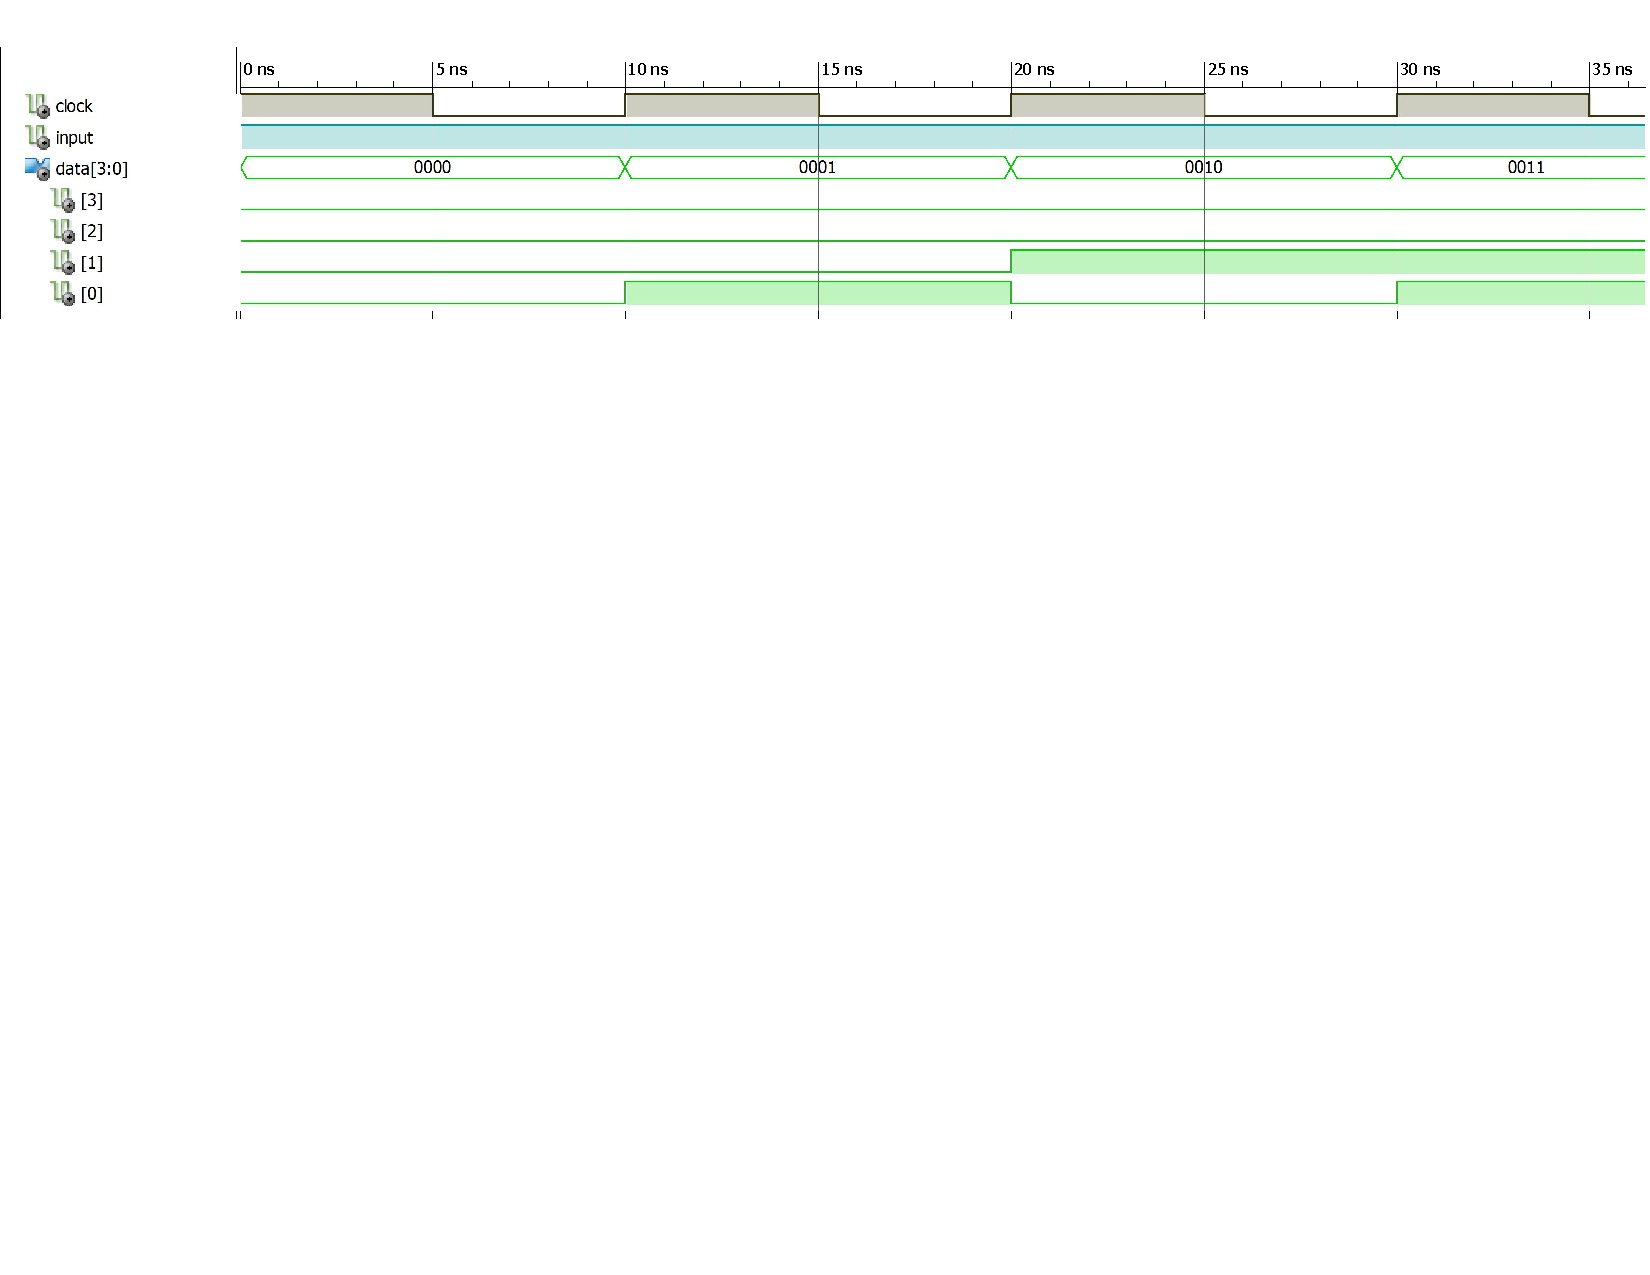
\includegraphics[width=.95\linewidth,  frame]{../Figures/5-1.pdf}
        \caption{}
        \label{fig:obs5-1}
        \end{subfigure}
        \begin{subfigure}{\linewidth}
            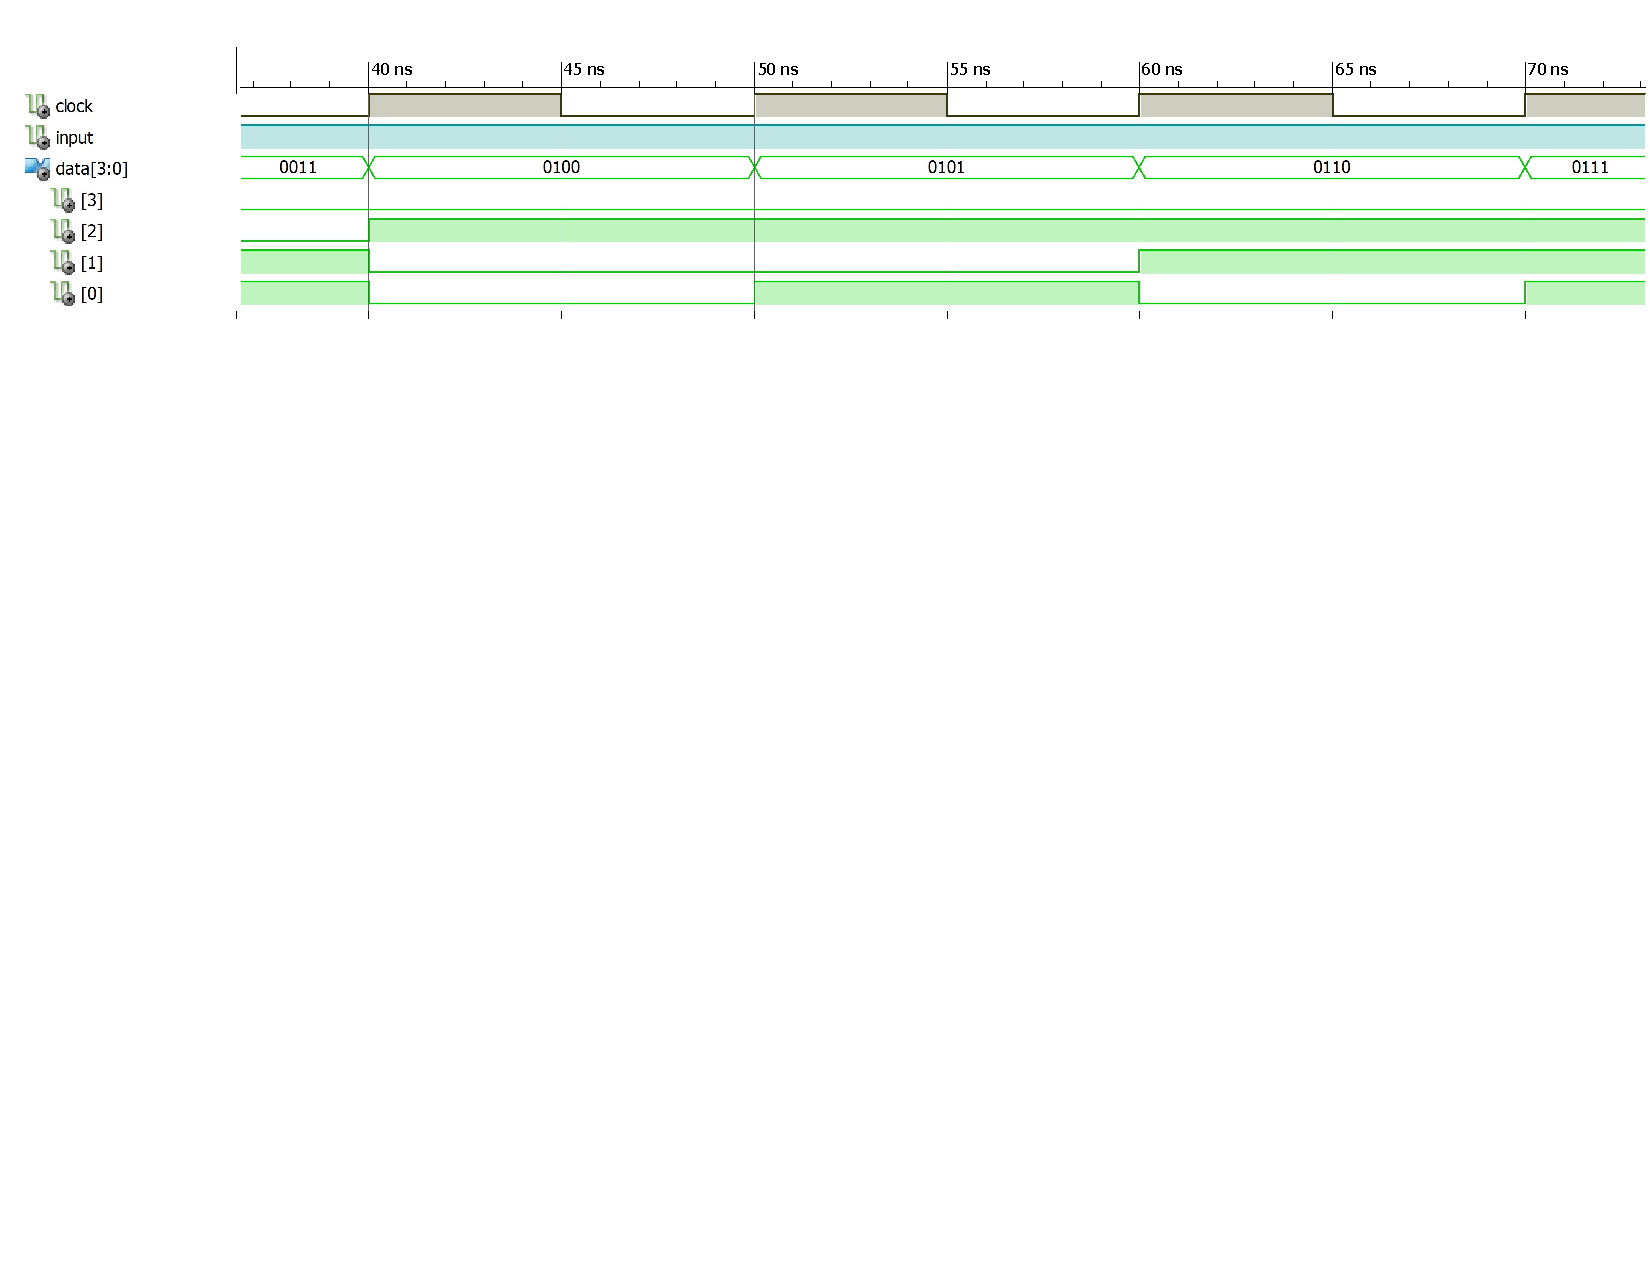
\includegraphics[width=.95\linewidth,  frame]{../Figures/5-2.pdf}
        \caption{}
        \label{fig:obs5-2}
        \end{subfigure}
        \begin{subfigure}{\linewidth}
            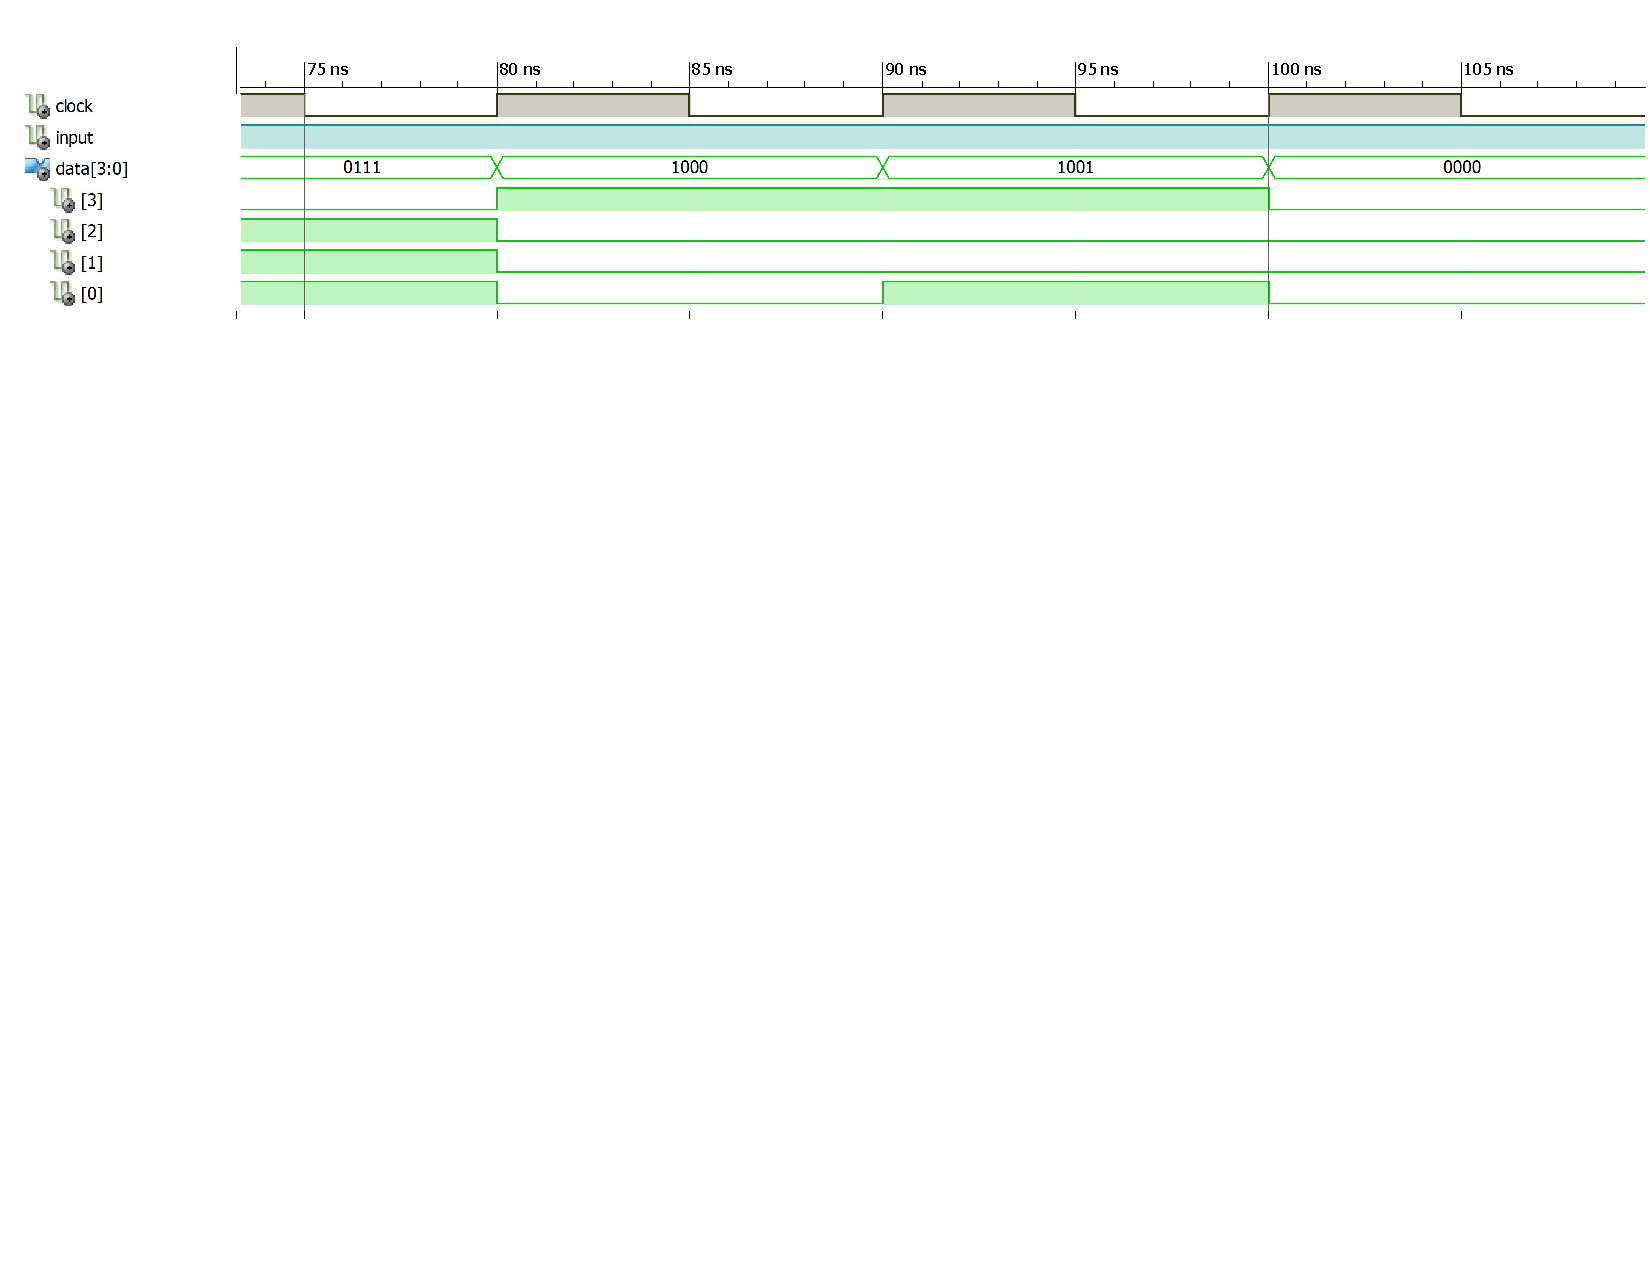
\includegraphics[width=.95\linewidth, frame]{../Figures/5-3.pdf}
        \caption{}
        \label{fig:obs5-3}
        \end{subfigure}
        \caption{Observed waveform for Problem 5}
        \label{fig:obs5}
    \end{figure}
    \begin{figure}[H]
        \centering
        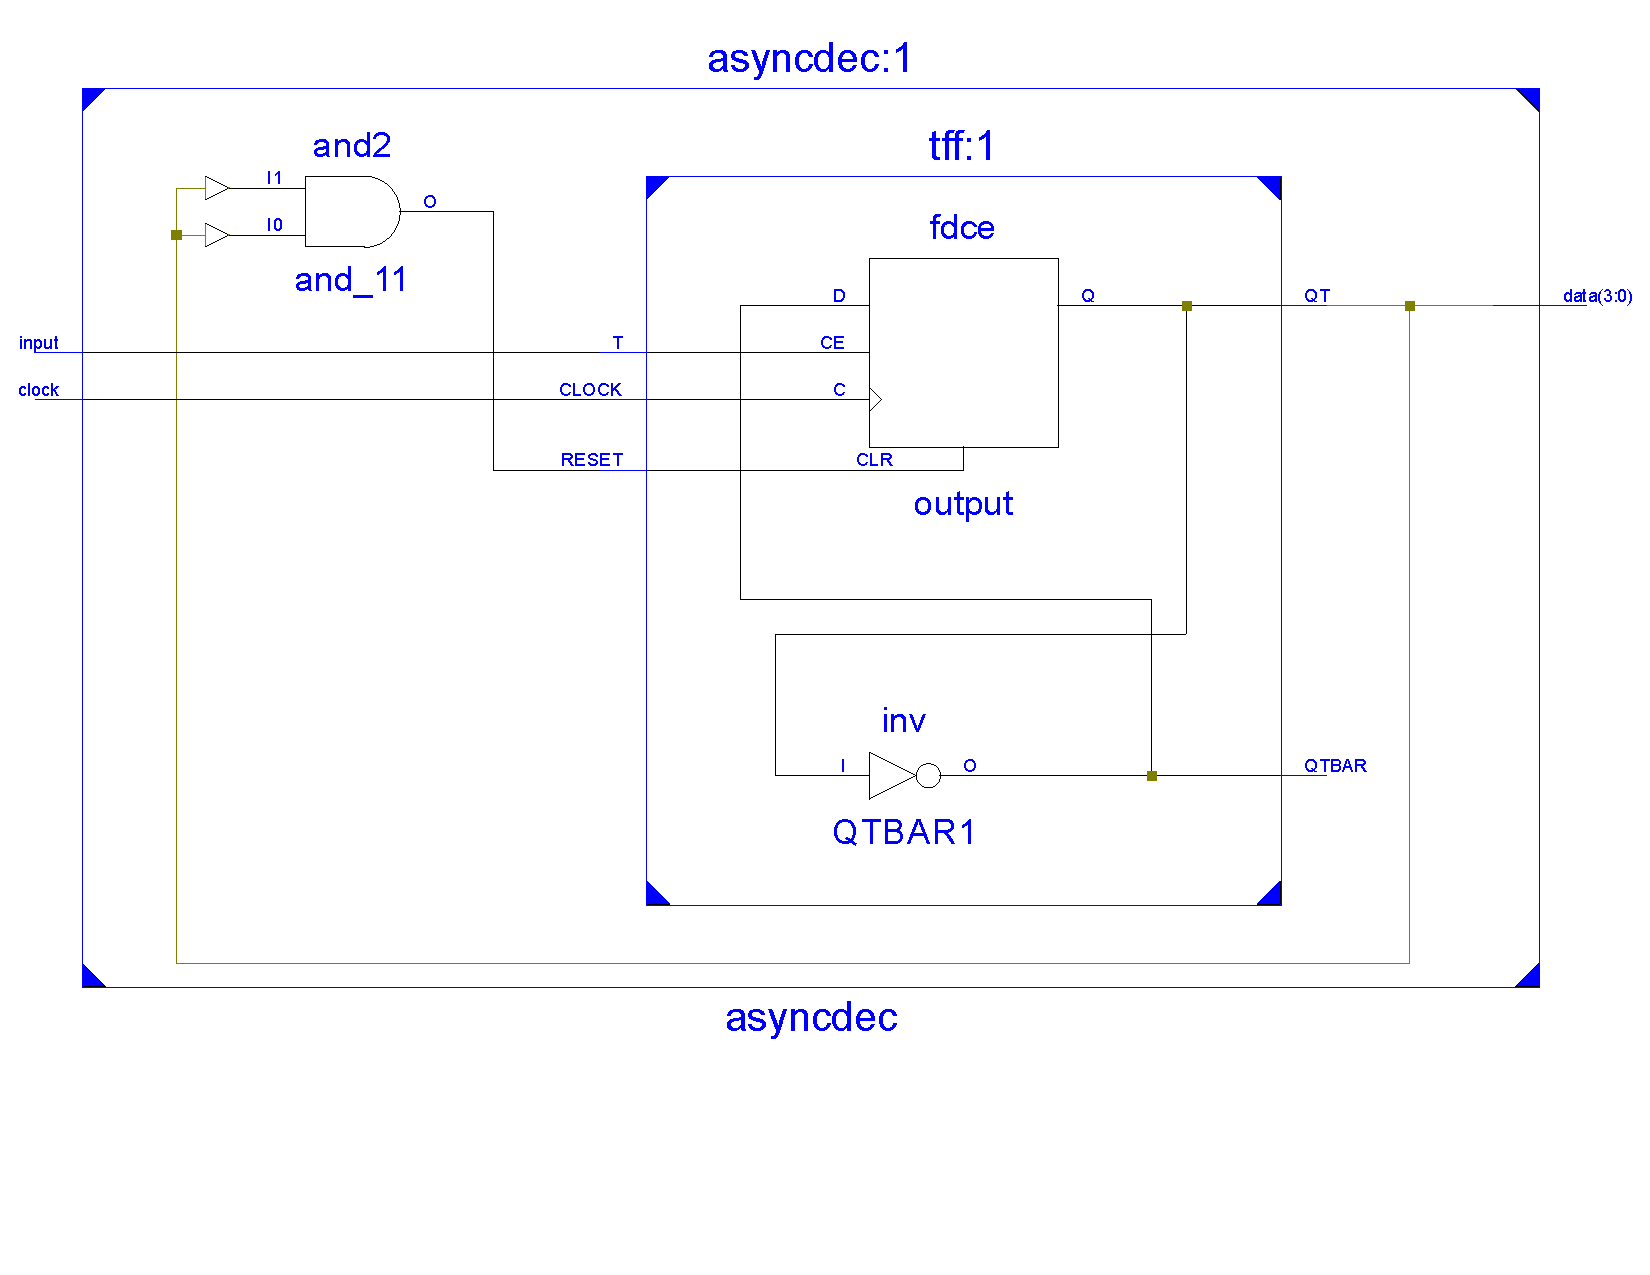
\includegraphics[scale=0.5]{../Figures/q5_ckt.pdf}
        \caption{Observed RTL schematic for Problem 5}
        \label{fig:rtl5}
    \end{figure}

    \subsubsection*{Problem 6}
    \begin{figure}[H]
        \centering
        \begin{subfigure}{\linewidth}
            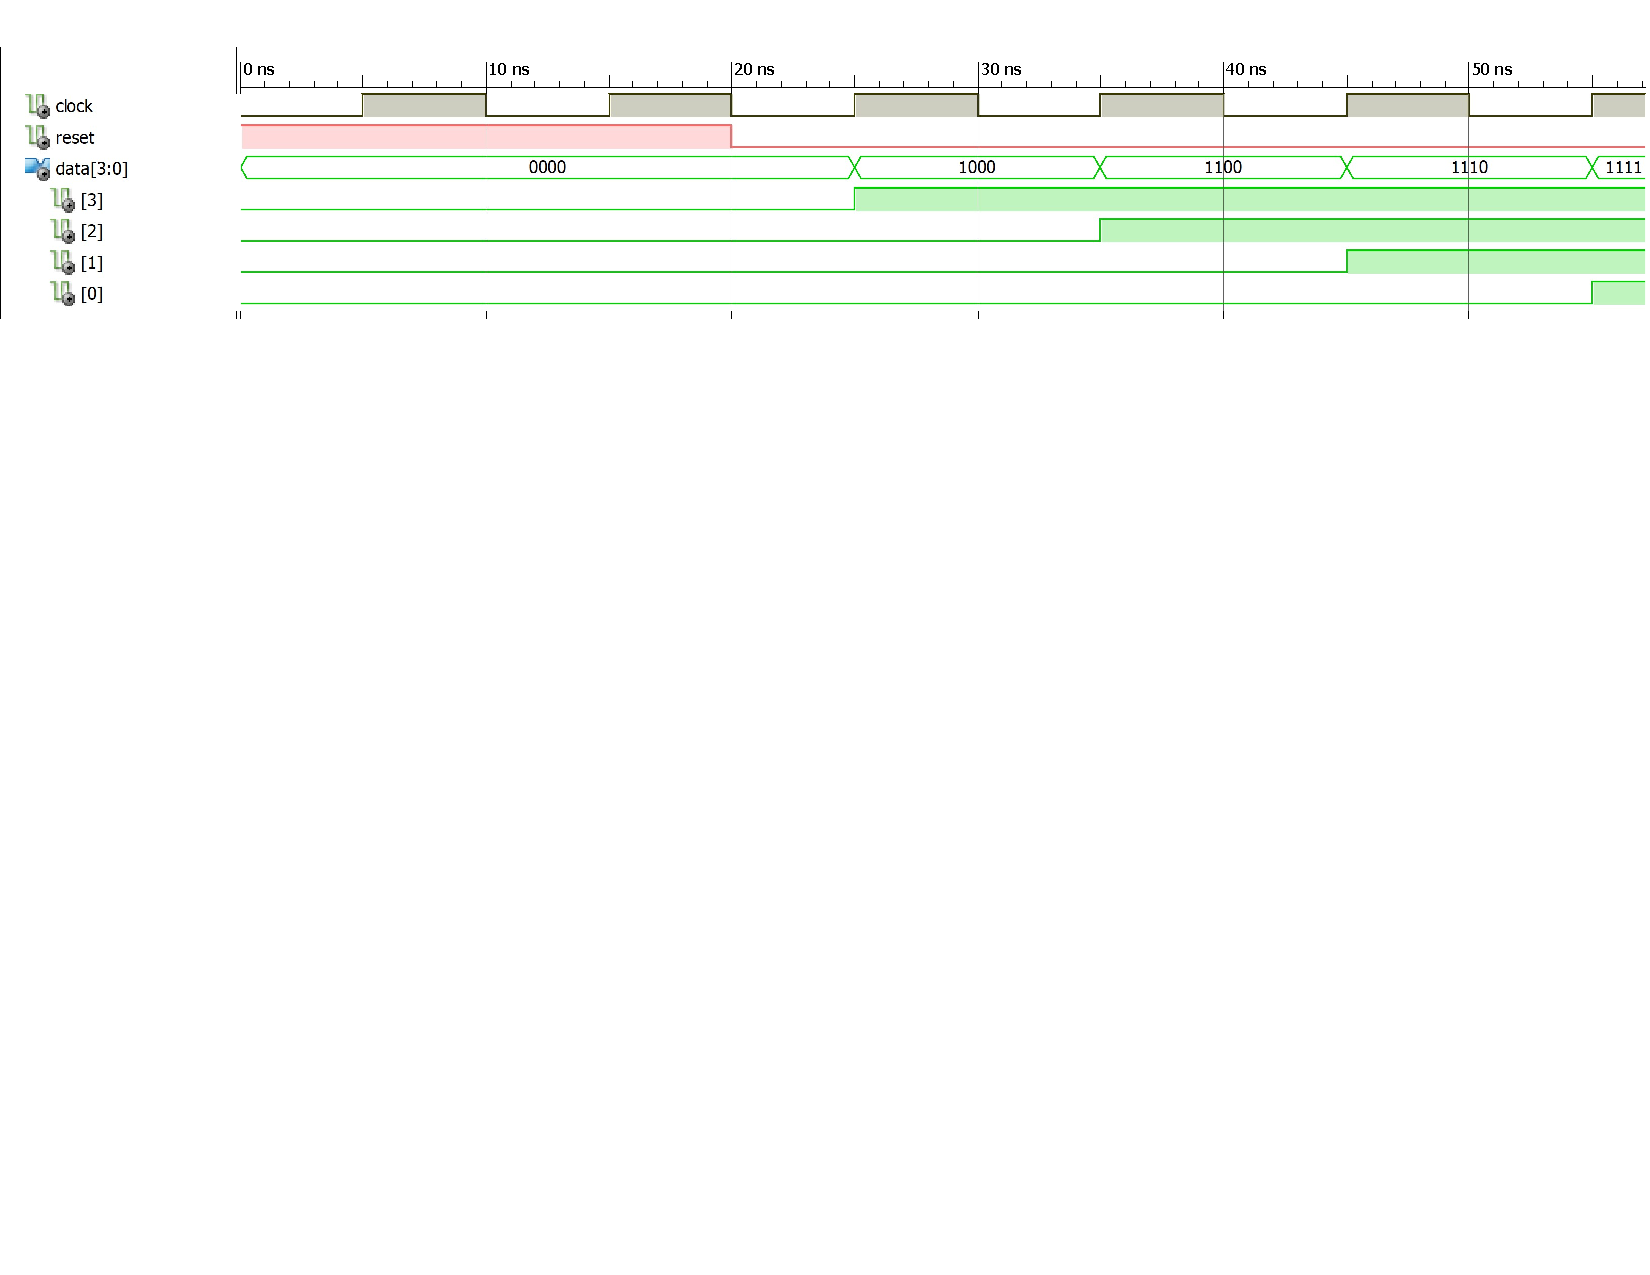
\includegraphics[width=.95\linewidth,  frame]{../Figures/6-1.pdf}
        \caption{}
        \label{fig:obs6-1}
        \end{subfigure}
        \begin{subfigure}{\linewidth}
            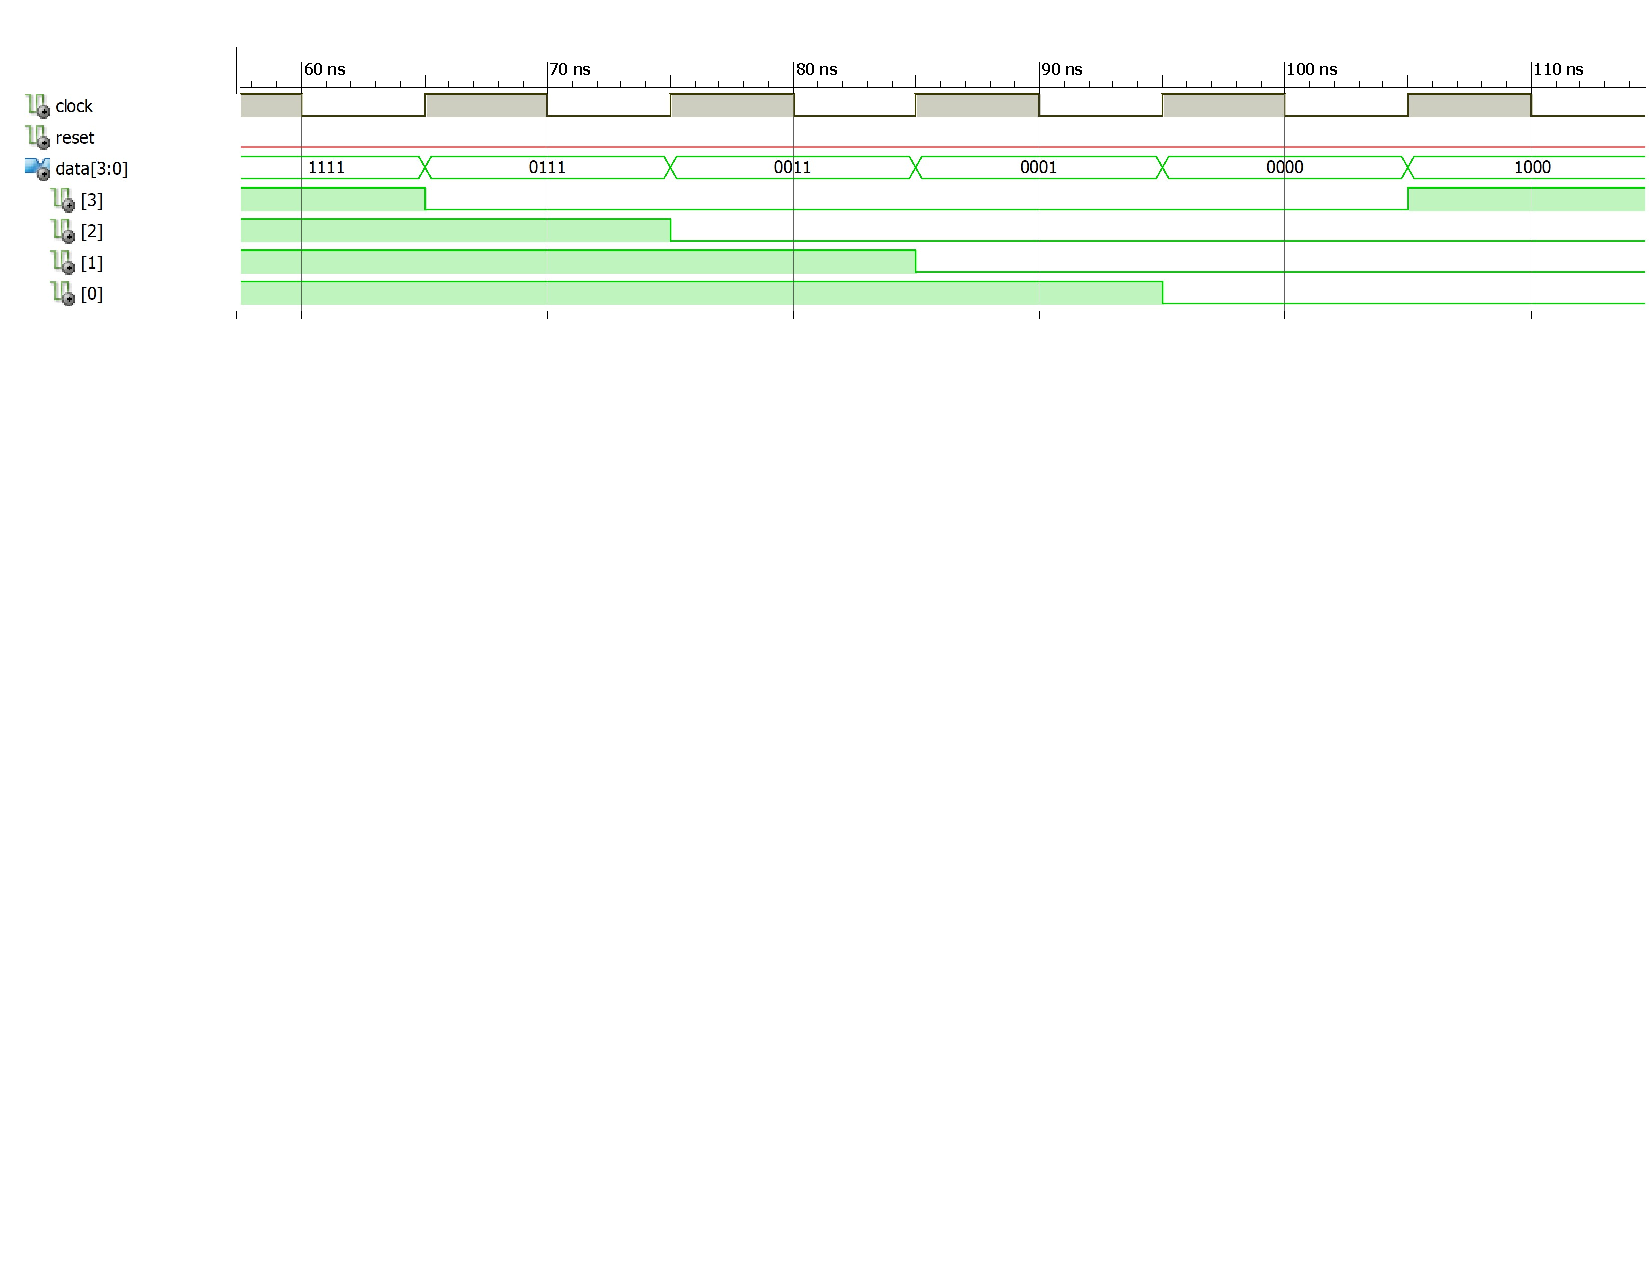
\includegraphics[width=.95\linewidth,  frame]{../Figures/6-2.pdf}
        \caption{}
        \label{fig:obs6-2}
        \end{subfigure}
        \caption{Observed waveform for Problem 6}
        \label{fig:obs6}
    \end{figure}
    \begin{figure}[H]
        \centering
        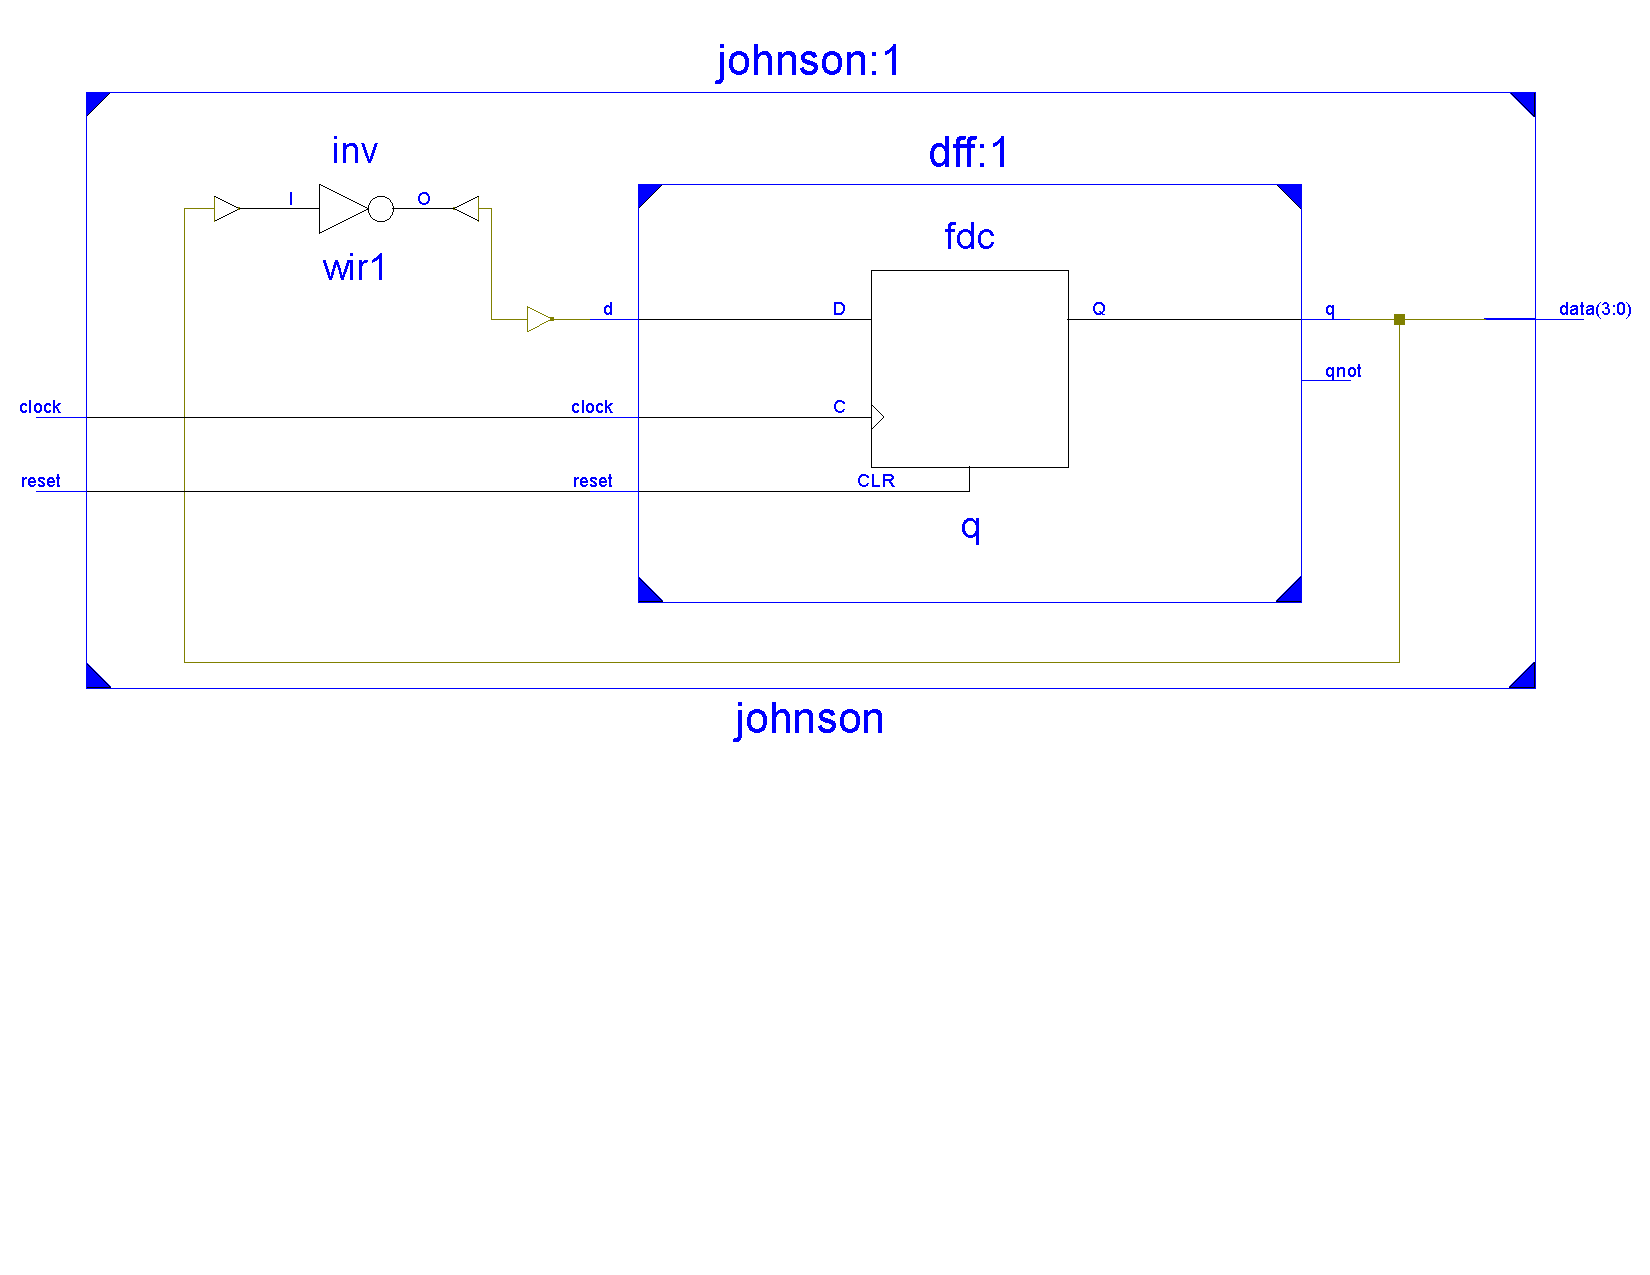
\includegraphics[scale=0.48]{../Figures/q6_ckt.pdf}
        \caption{Observed RTL schematic for Problem 6}
        \label{fig:rtl6}
    \end{figure}

    \subsubsection*{Problem 7}
    \begin{figure}[H]
        \centering
        \begin{subfigure}{\linewidth}
            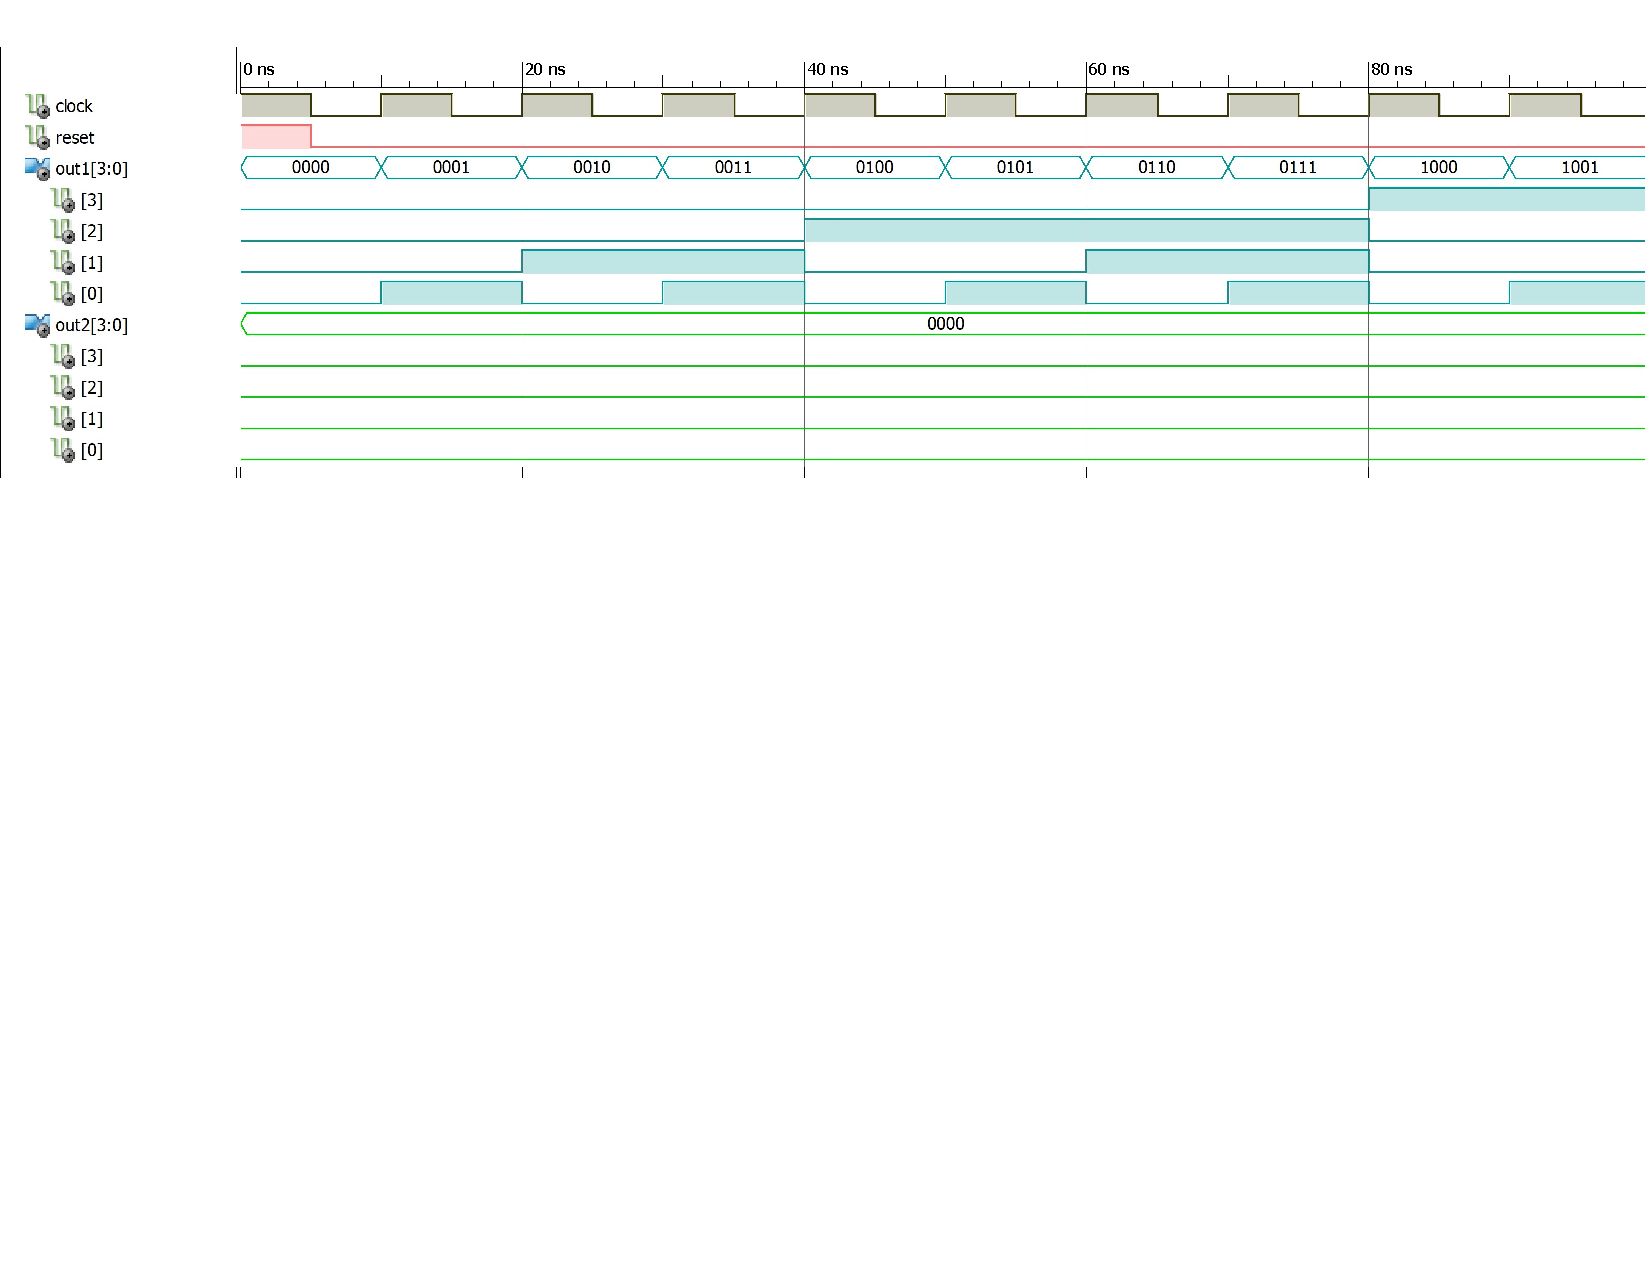
\includegraphics[width=.95\linewidth, frame]{../Figures/7-1.pdf}
        \caption{}
        \label{fig:obs7-1}
        \end{subfigure}
        \caption{Observed waveform for Problem 7}
        \label{fig:obs7}
    \end{figure}
    \begin{figure}[H]\ContinuedFloat
        \centering
        \foreach \i in {2,3,4,5}
        {
            \begin{subfigure}{\linewidth}
            \includegraphics[width=.95\linewidth, frame]{../Figures/7-\i.pdf}
        \caption{}
        \label{fig:obs7-\i}
        \end{subfigure}
        }
        \caption*{Figure~\ref{fig:obs7}:~Observed waveform for Problem 7 (continued)}
    \end{figure}
    \begin{figure}[H]\ContinuedFloat
        \centering
        \foreach \i in {6,7,8,9}
        {
            \begin{subfigure}{\linewidth}
            \includegraphics[width=.95\linewidth, frame]{../Figures/7-\i.pdf}
        \caption{}
        \label{fig:obs7-\i}
        \end{subfigure}
        }
        \caption*{Figure~\ref{fig:obs7}:~Observed waveform for Problem 7 (continued)}
    \end{figure}
    \begin{figure}[H]\ContinuedFloat
        \centering
            \begin{subfigure}{\linewidth}
            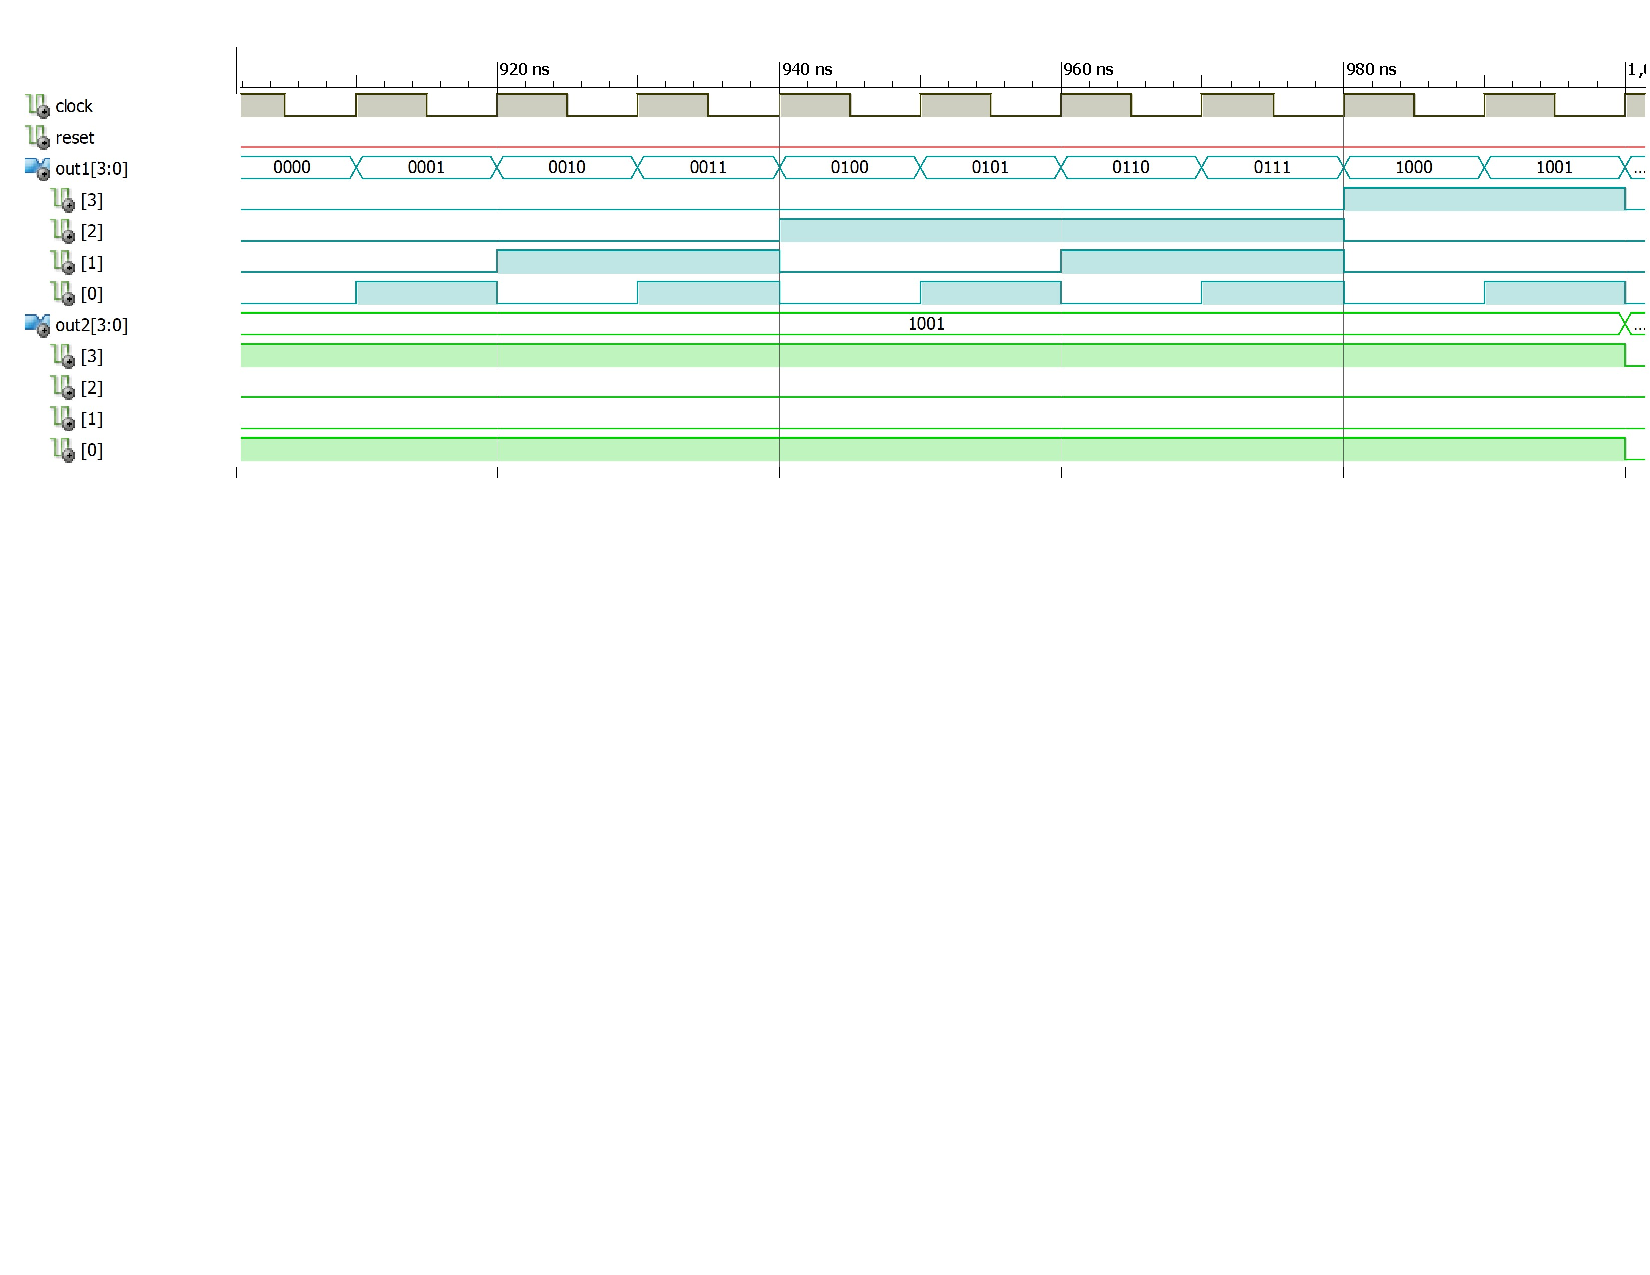
\includegraphics[width=.95\linewidth, frame]{../Figures/7-10.pdf}
        \caption{}
        \label{fig:obs7-10}
        \end{subfigure}
        \caption*{Figure~\ref{fig:obs7}:~Observed waveform for Problem 7 (continued)}
    \end{figure}
    \begin{figure}[H]
        \centering
        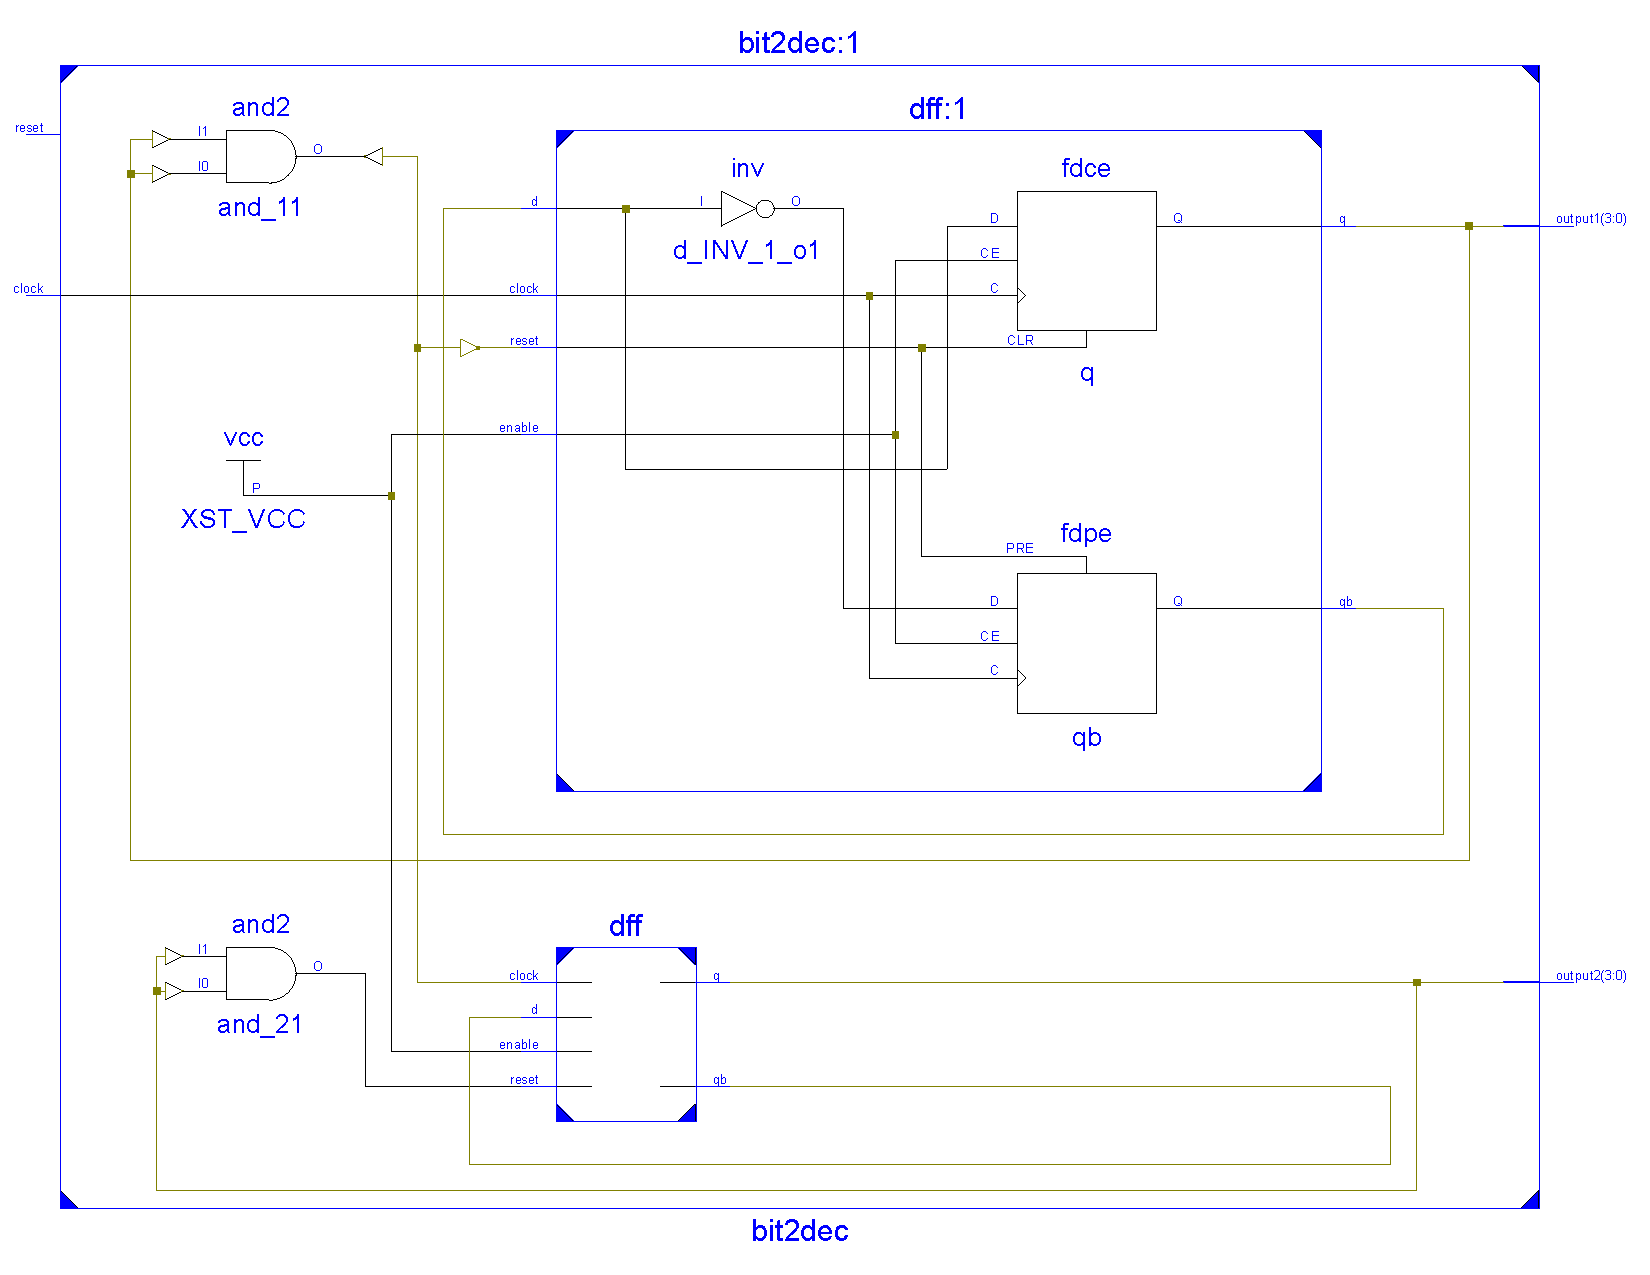
\includegraphics[scale=0.5]{../Figures/q7_ckt.pdf}
        \caption{Observed RTL schematic for Problem 7}
        \label{fig:rtl7}
    \end{figure}
    \section{Discussion}
    In this lab experiment, various programs related to sequential logic circuits were written in VHDL. Problems related to JK and T flip flops using D flip flops and basic gates, SISO register, synchronous up, asynchronous decade, johnson and two bit BCD counters allowed us to be familiar with VHDL programming concepts that are involved while designing a FPGA. The waveforms are results of ISim, a full-featured HDL simulator which was initiated by test bench programs written in VHDL. The test bench codes have been included with this report as per the instructions. RTL schematics of the combinational circuits have been included with this report since it provides a clear idea of the various modules that are used while in a complex circuit.
    \printbibliography[heading=bibintoc,title={Additional References},notcategory=cited]
\end{document}